
Data to background comparison of variables from the kinematic fitted objects after kinematic 
fit selection are shown in Figures~\ref{fig:kfitPlot1},~\ref{fig:kfitPlot2}, and~\ref{fig:kfitPlot3}. 
There is also a good agreement between data and simulation within the statistical and systematic 
uncertainties. Here also we see a similar disagreement for the higher value of \pt and \MET as
we have after \PQb jet selection described in Section~\ref{s:secEvtSel}.

%After KinFit: Pt_lep, Eta_lep, Pt_jets
\begin{figure}
    \centering  
    \subfigure[\pt of muon]{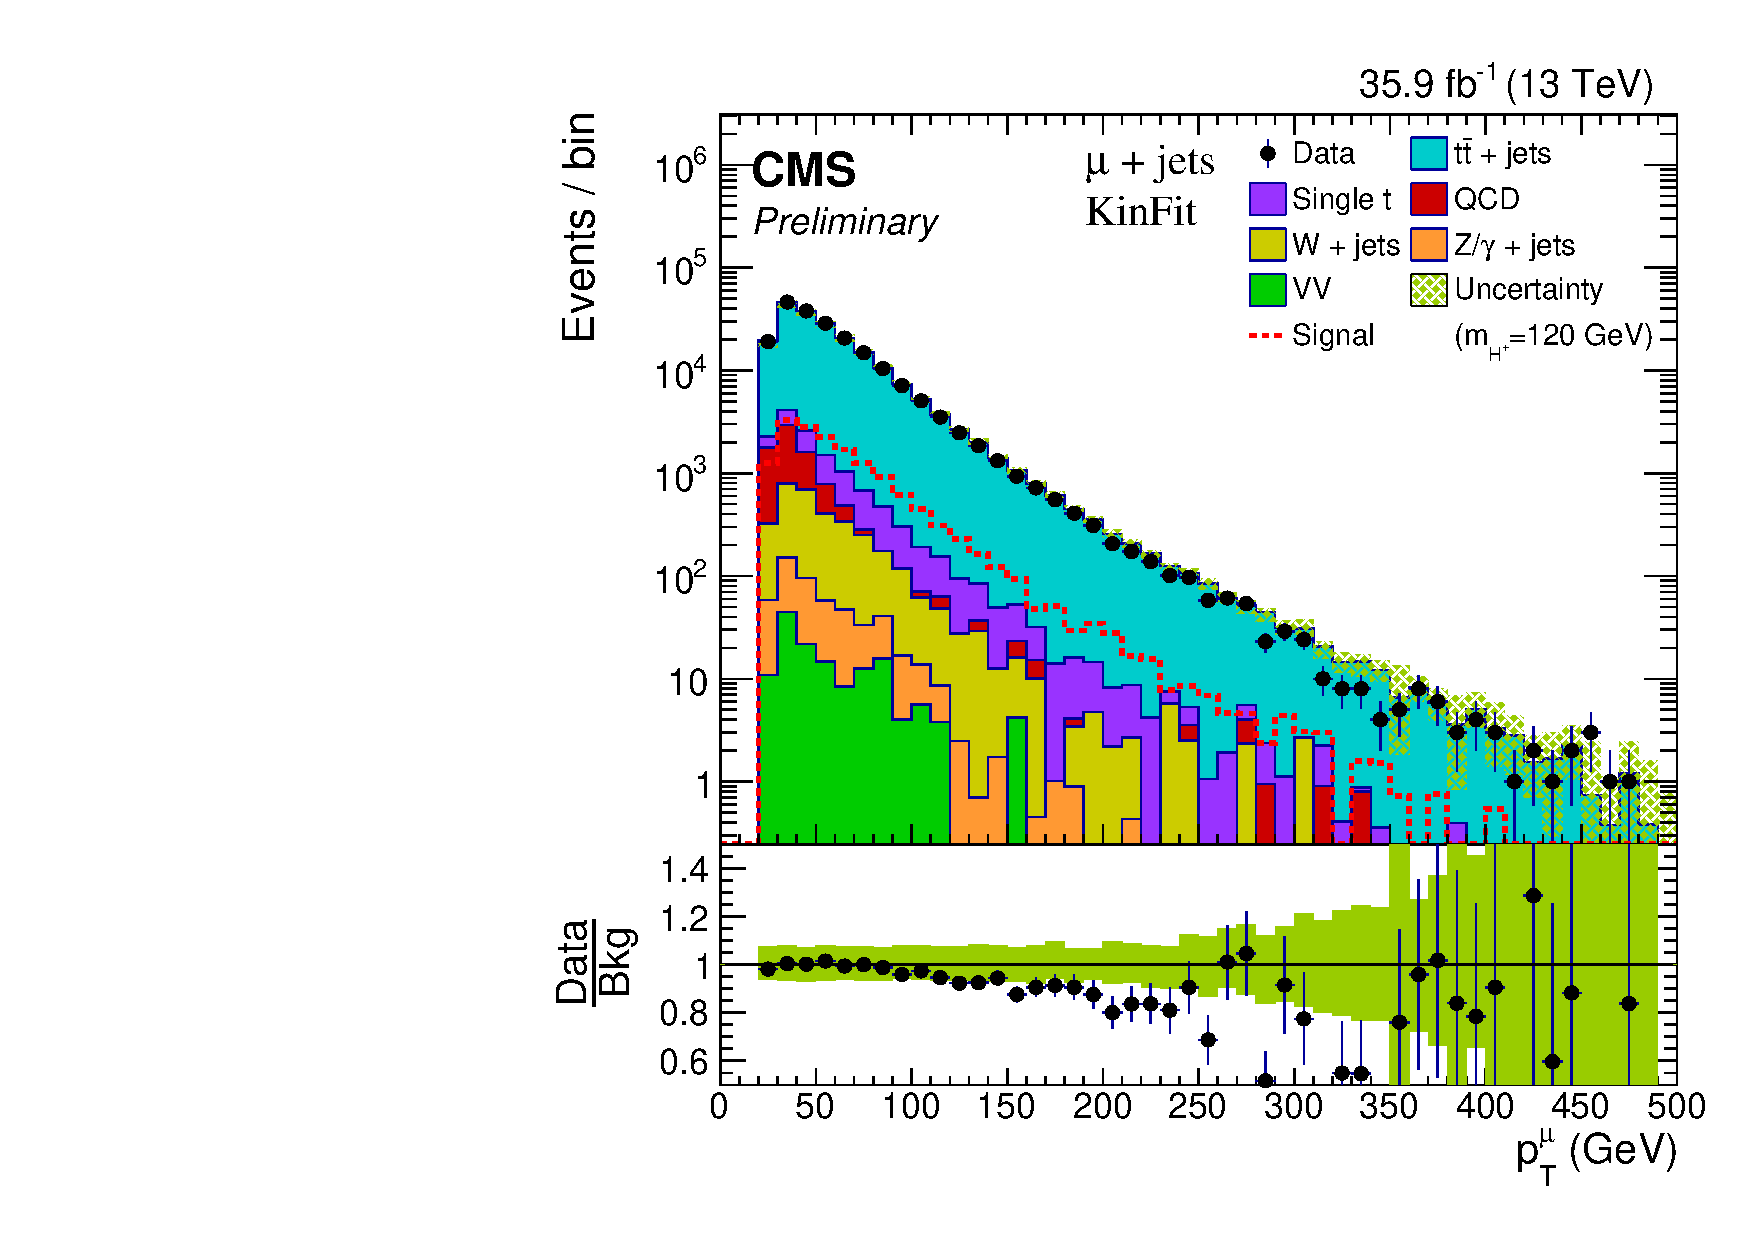
\includegraphics[width=0.40\linewidth]{Image/Muon/KinFit/pt_mu_muKinFit.pdf}}
    \subfigure[\pt of electron]{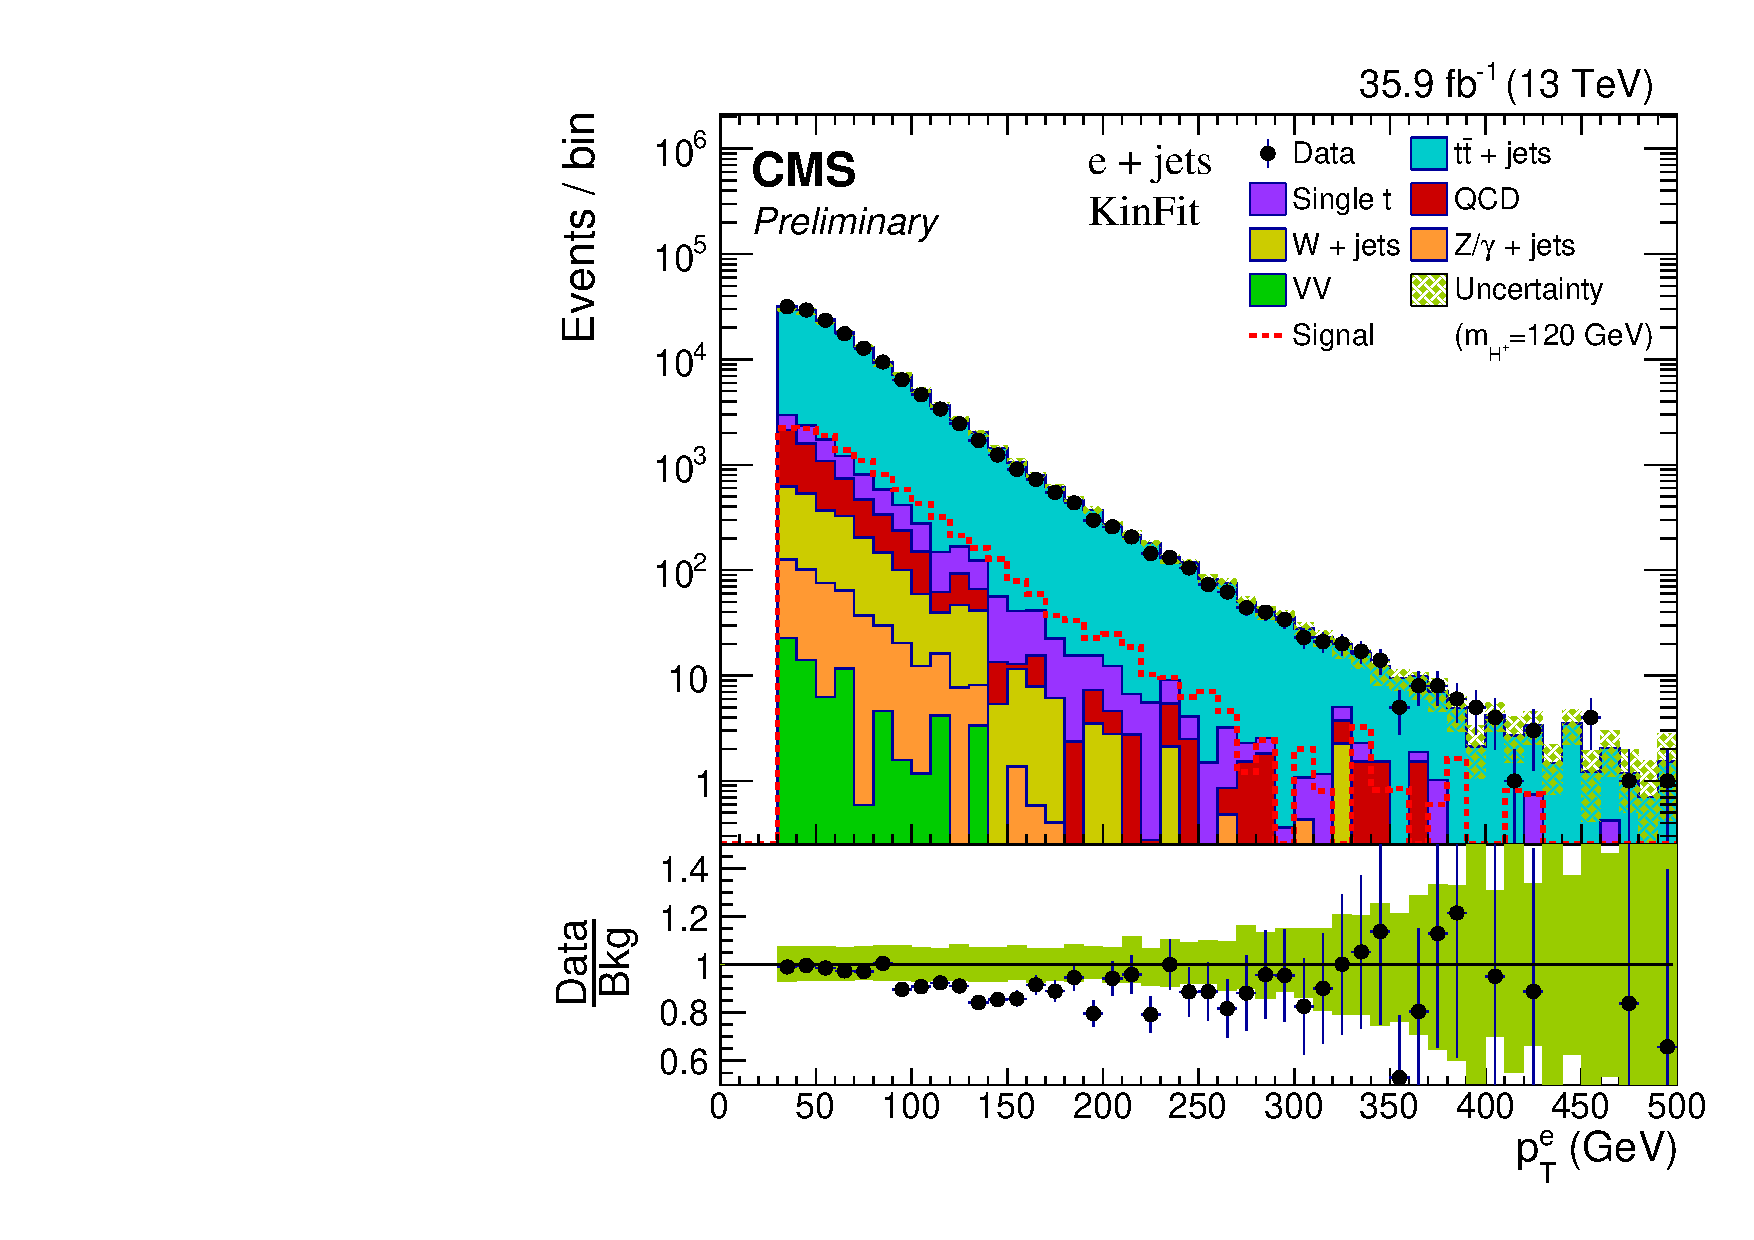
\includegraphics[width=0.40\linewidth]{Image/Electron/KinFit/pt_ele_eleKinFit.pdf}}
    \vfil
    \subfigure[$\eta$ of muon]{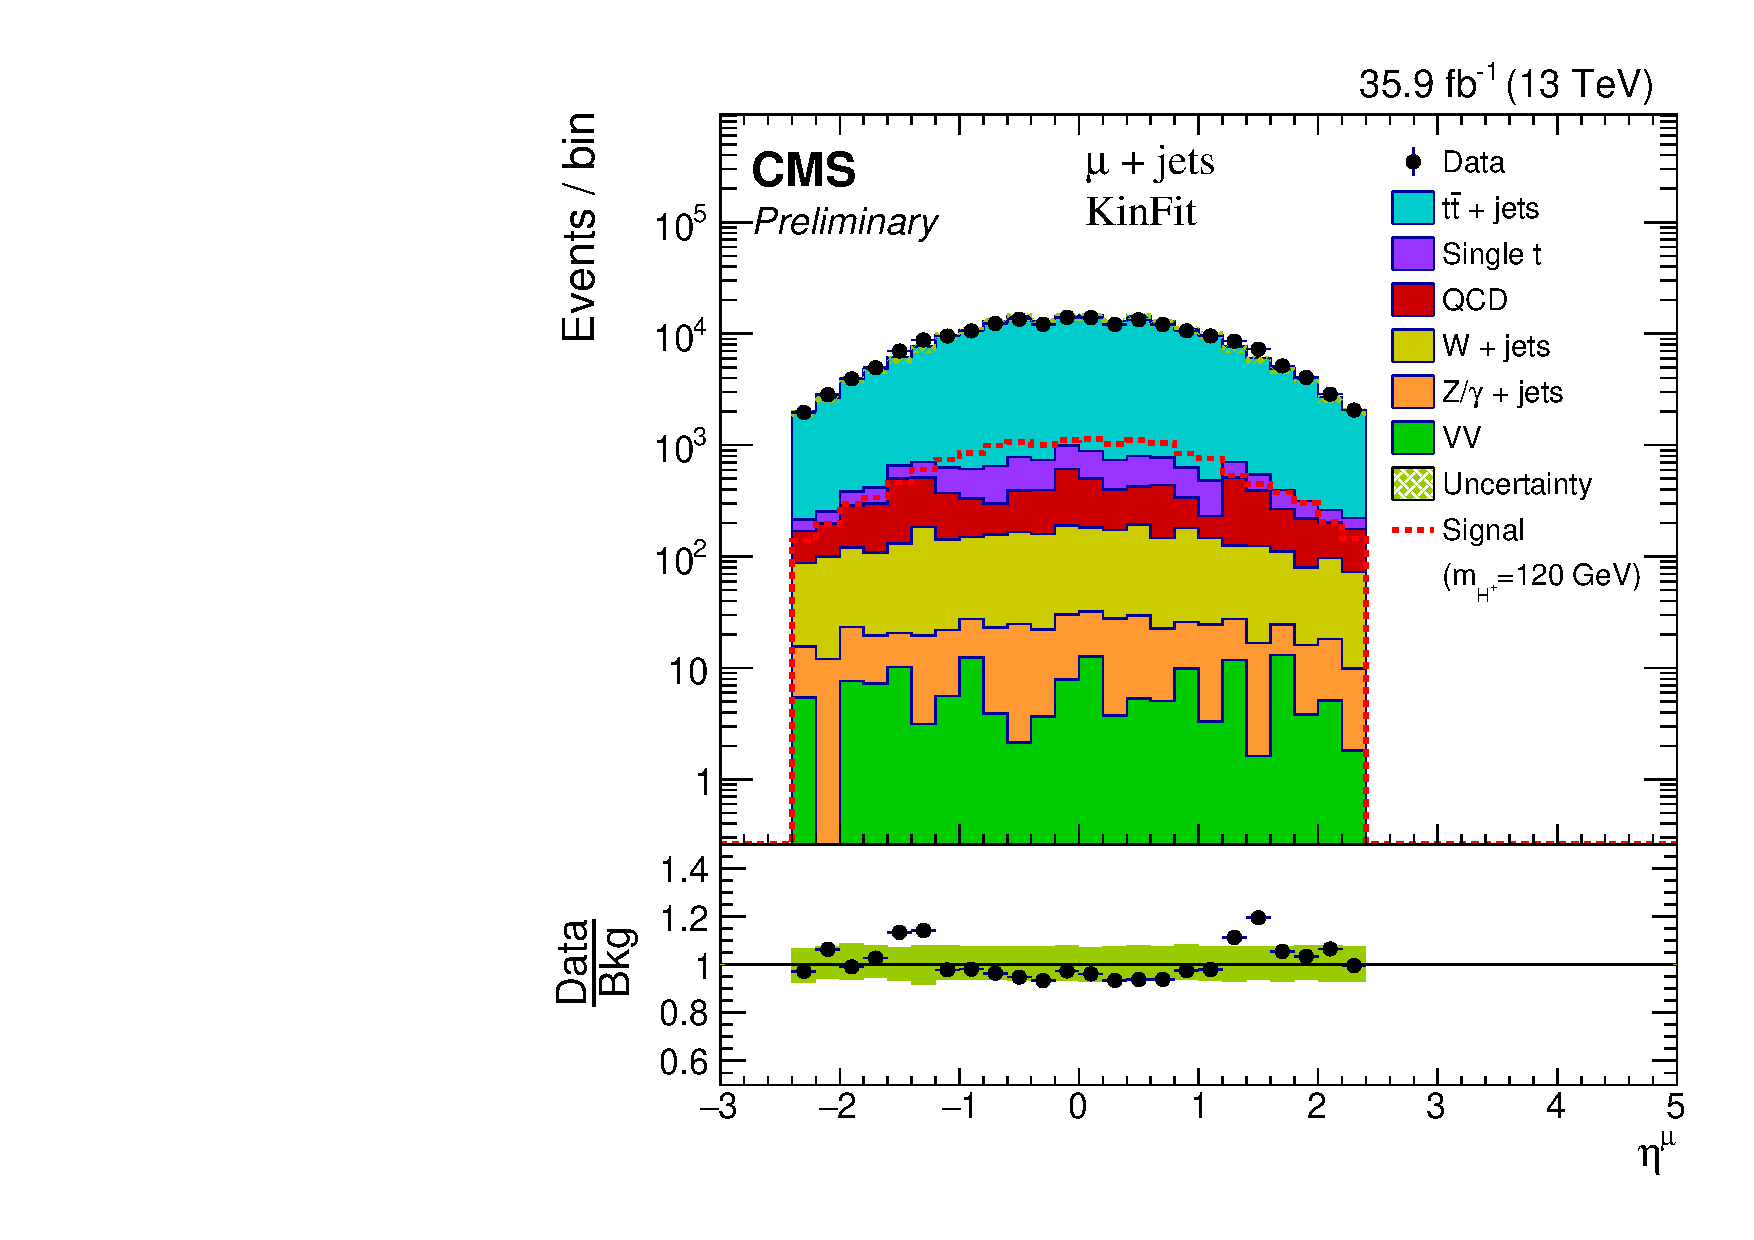
\includegraphics[width=0.40\linewidth]{Image/Muon/KinFit/eta_mu_muKinFit.pdf}}
    \subfigure[$\eta$ of electron]{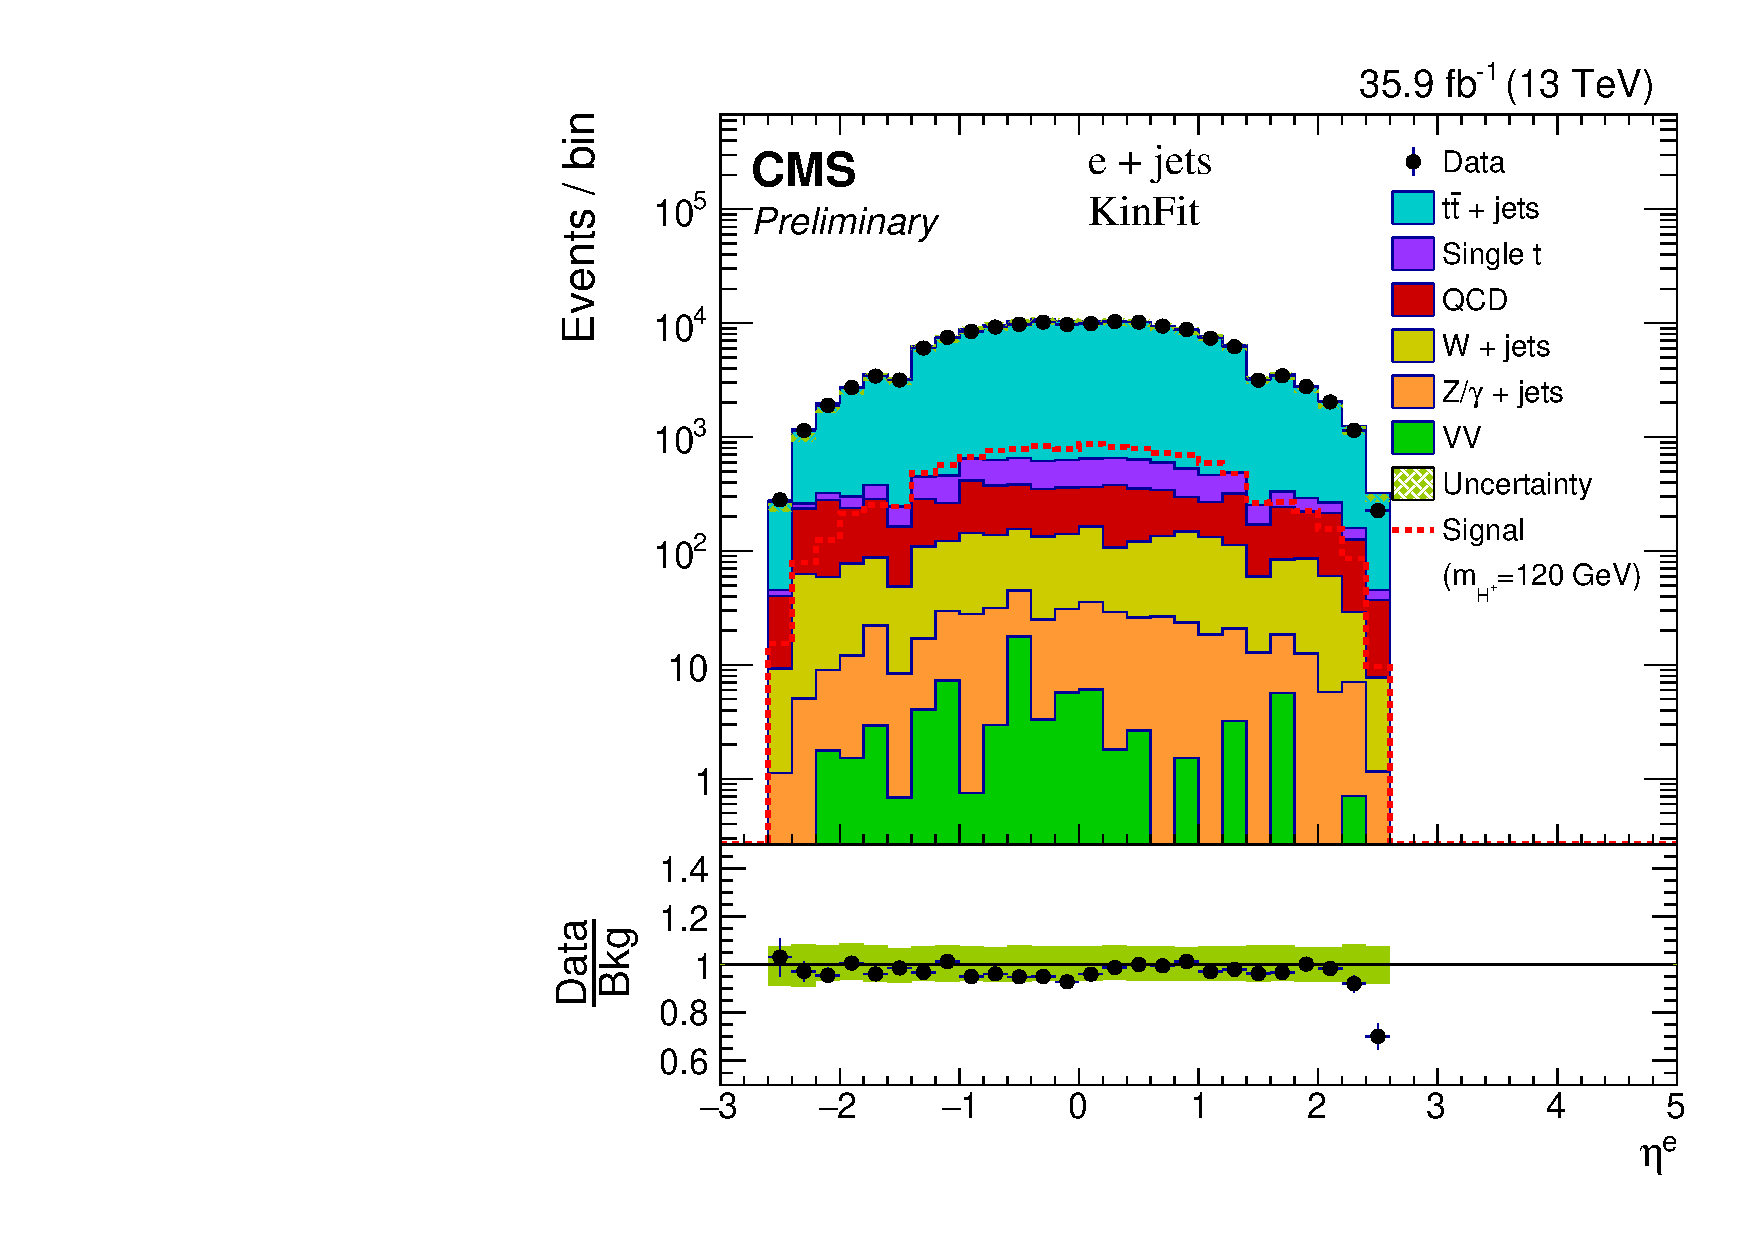
\includegraphics[width=0.40\linewidth]{Image/Electron/KinFit/eta_ele_eleKinFit.pdf}}
    \vfil
    \subfigure[\pt of jets]{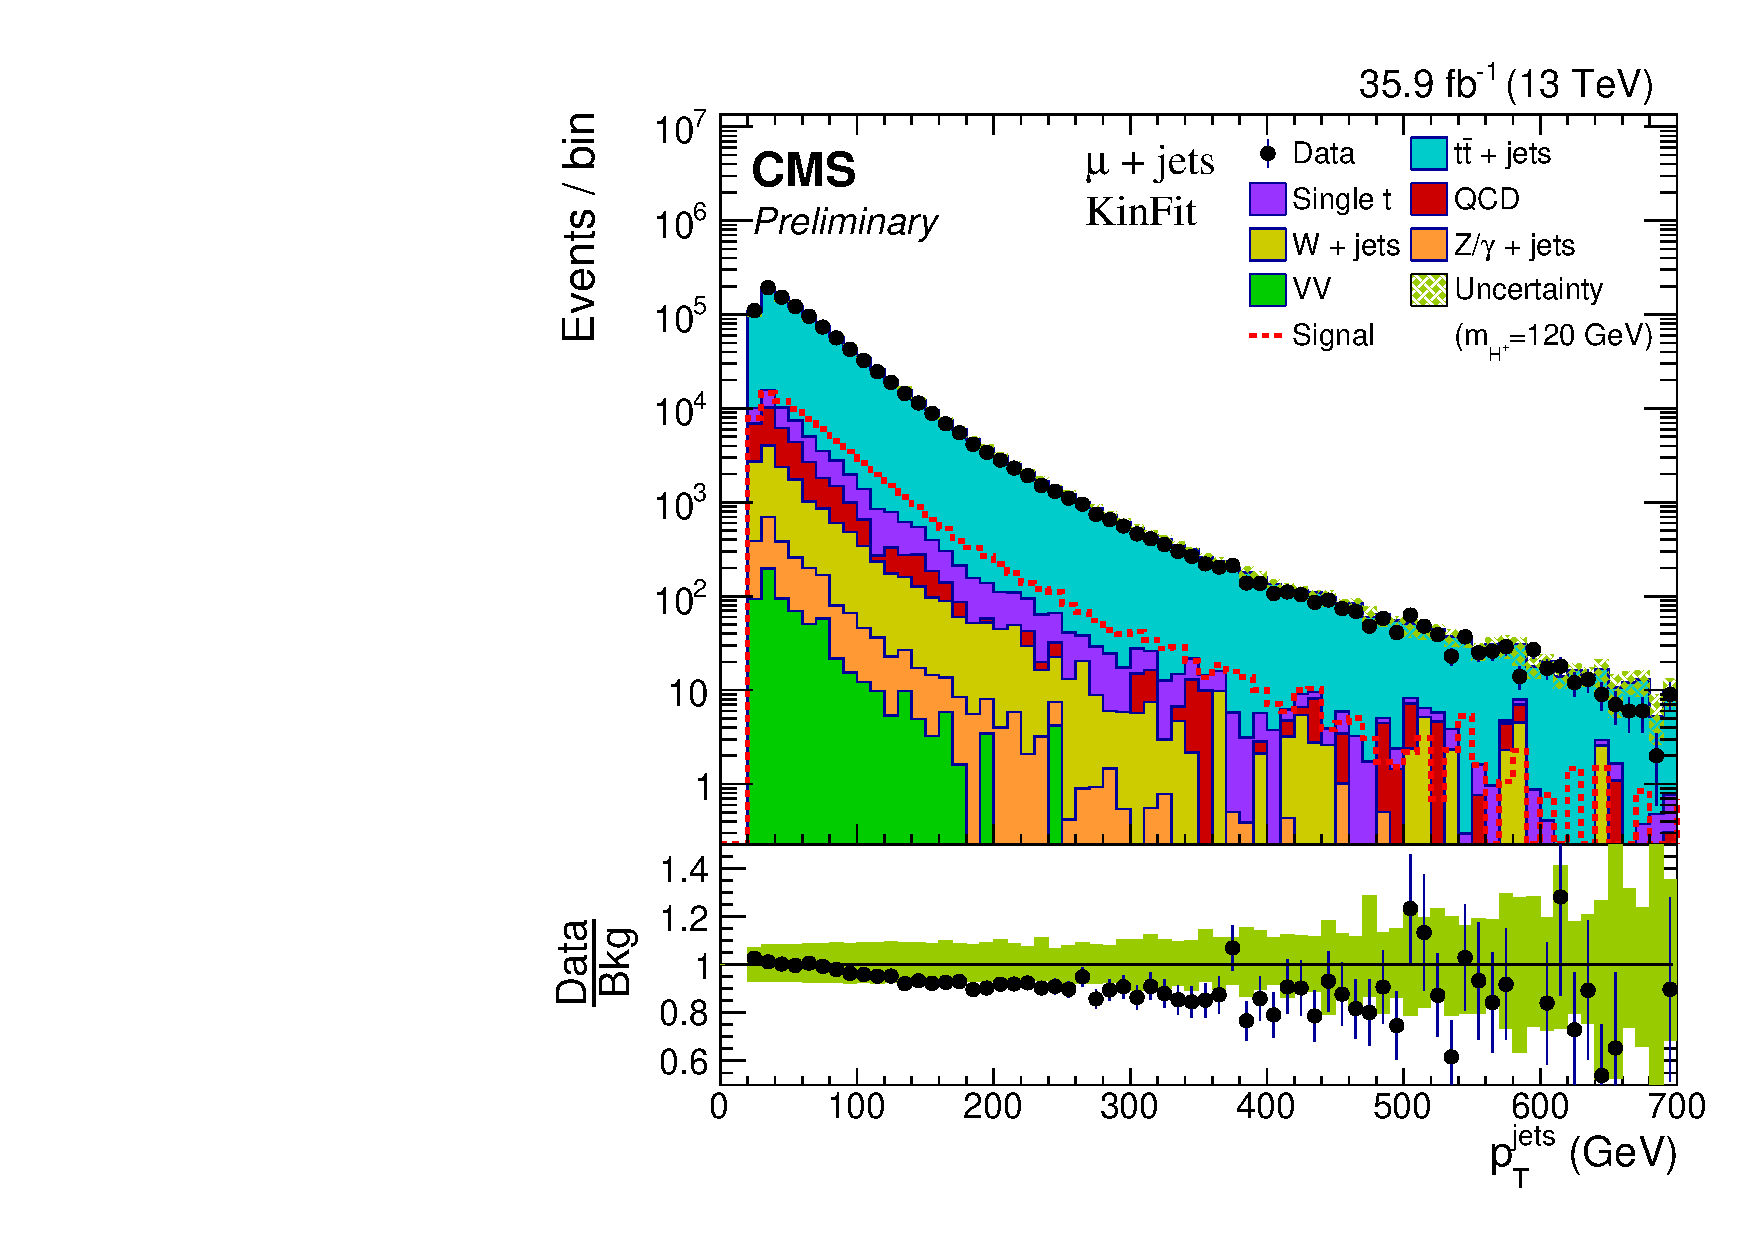
\includegraphics[width=0.40\linewidth]{Image/Muon/KinFit/pt_jet_muKinFit.pdf}}
    \subfigure[\pt of jets]{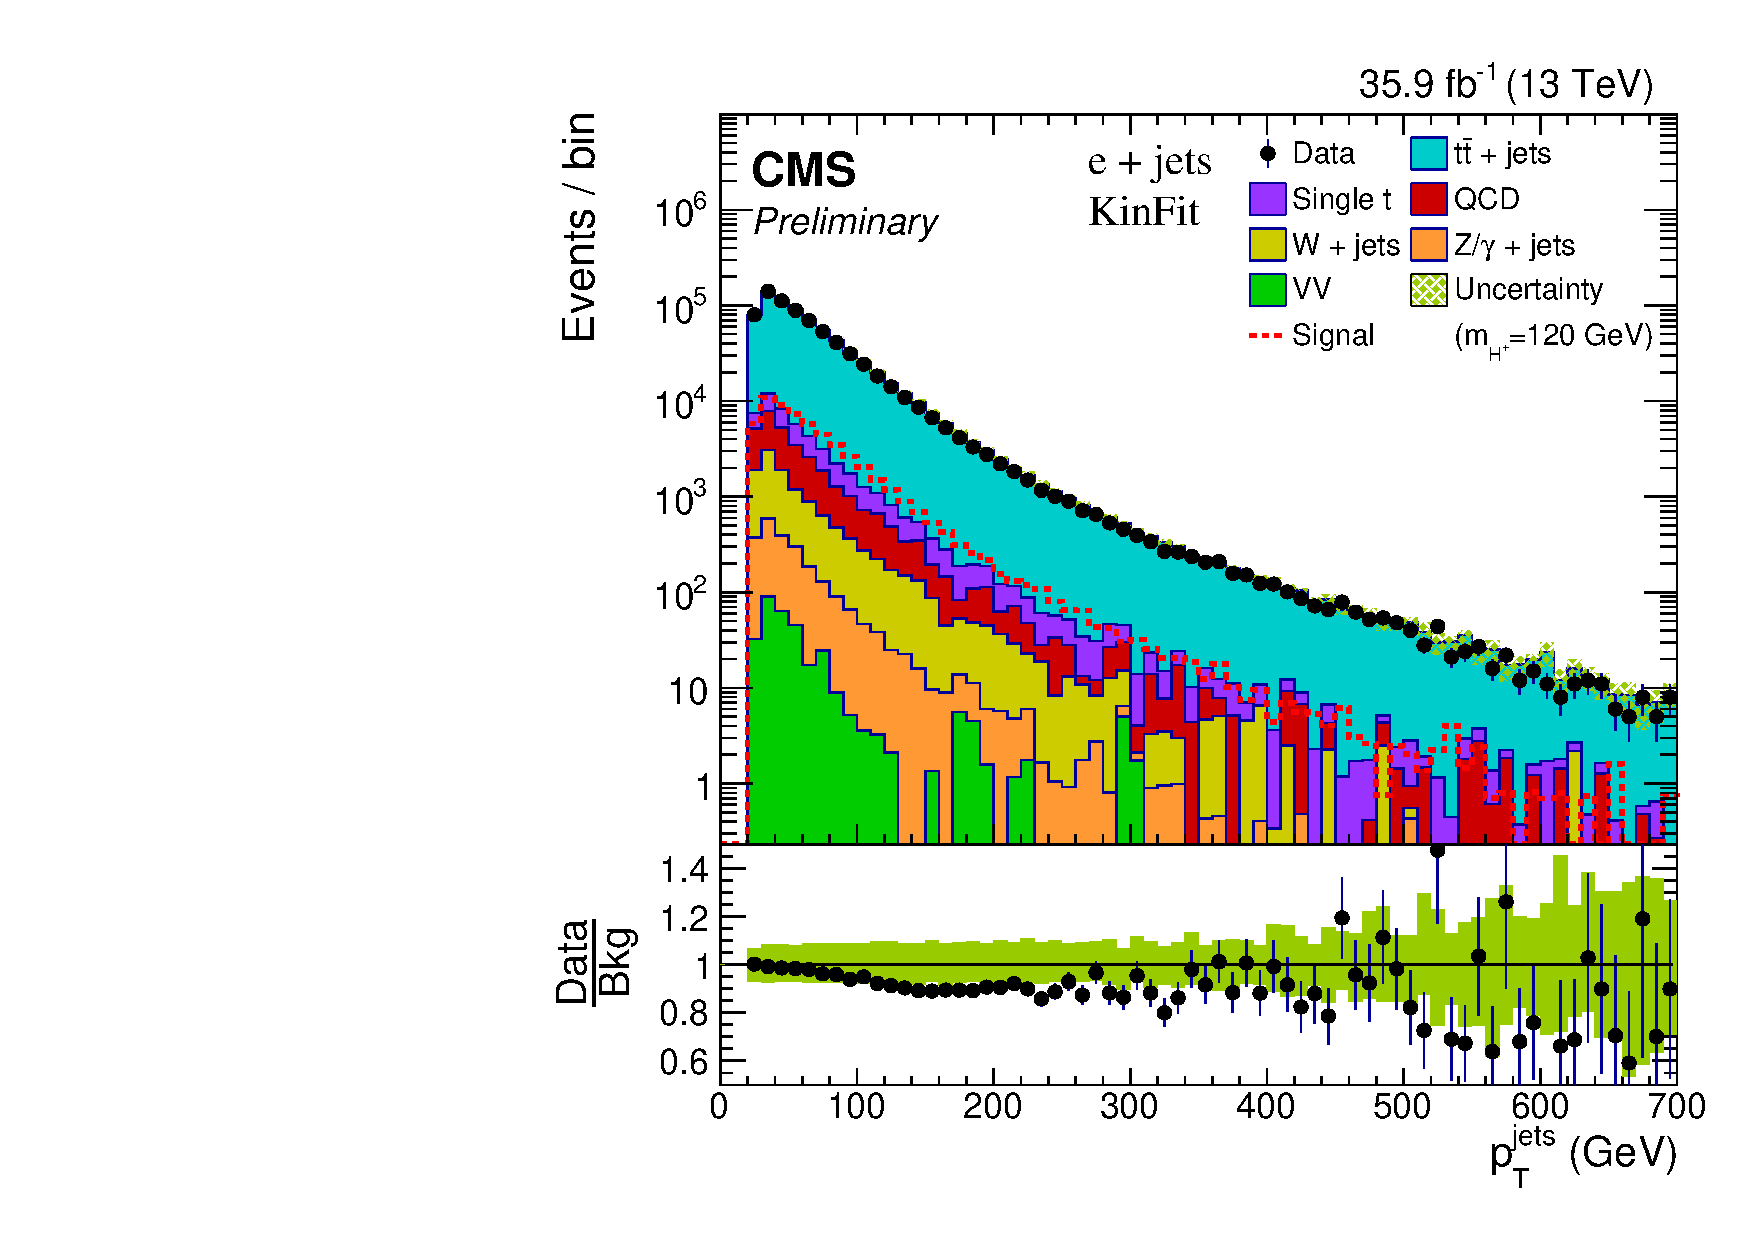
\includegraphics[width=0.40\linewidth]{Image/Electron/KinFit/pt_jet_eleKinFit.pdf}}
    \caption{Distribution of $\pt, \eta$ of kinematic fitted lepton and $\pt$ of jets
    after kinematic fit selection for \mujets and \ejets channel.}
    \label{fig:kfitPlot1}
\end{figure}

%After KinFit:Eta_jets , N_jets, N_bjets
\begin{figure}
    \centering  
    \subfigure[$\eta$ of jets]{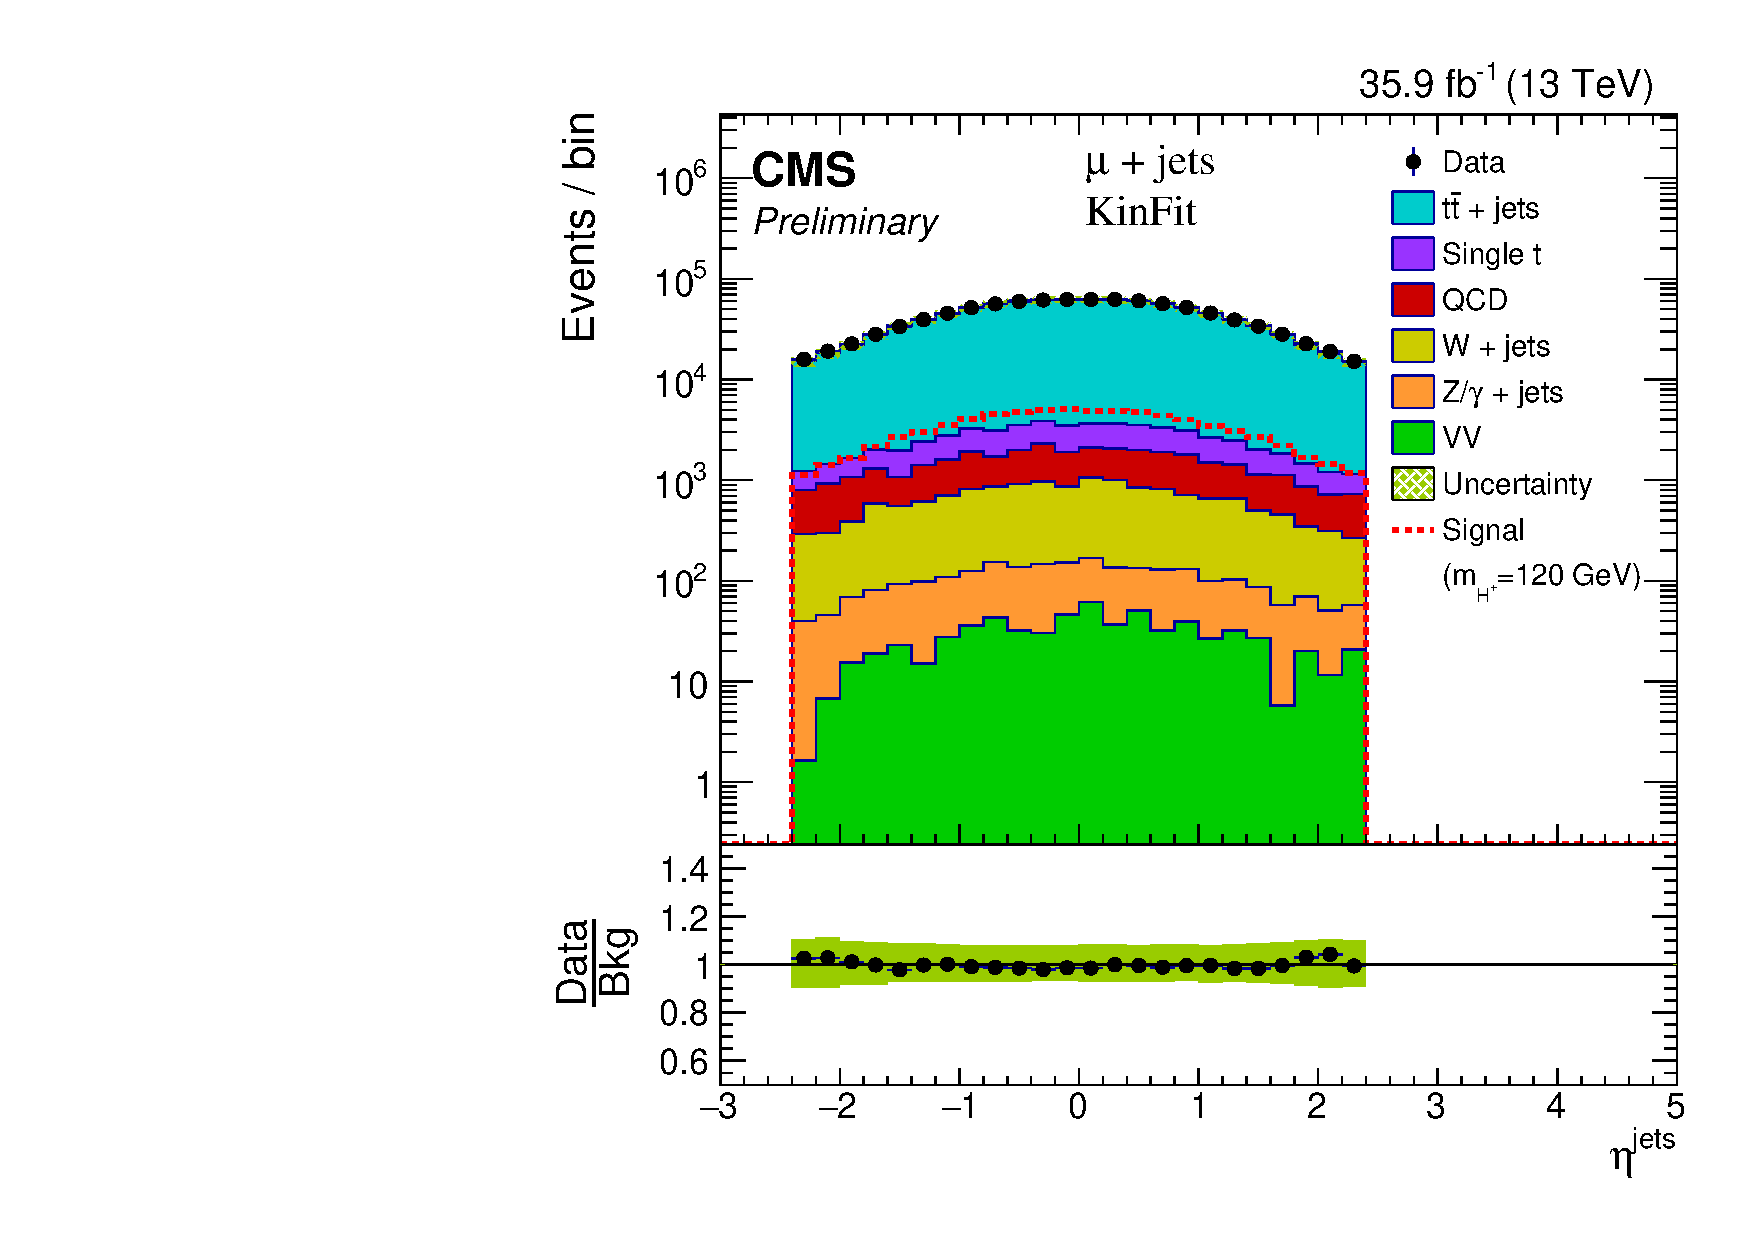
\includegraphics[width=0.40\linewidth]{Image/Muon/KinFit/eta_jet_muKinFit.pdf}}
    \subfigure[$\eta$ of jets]{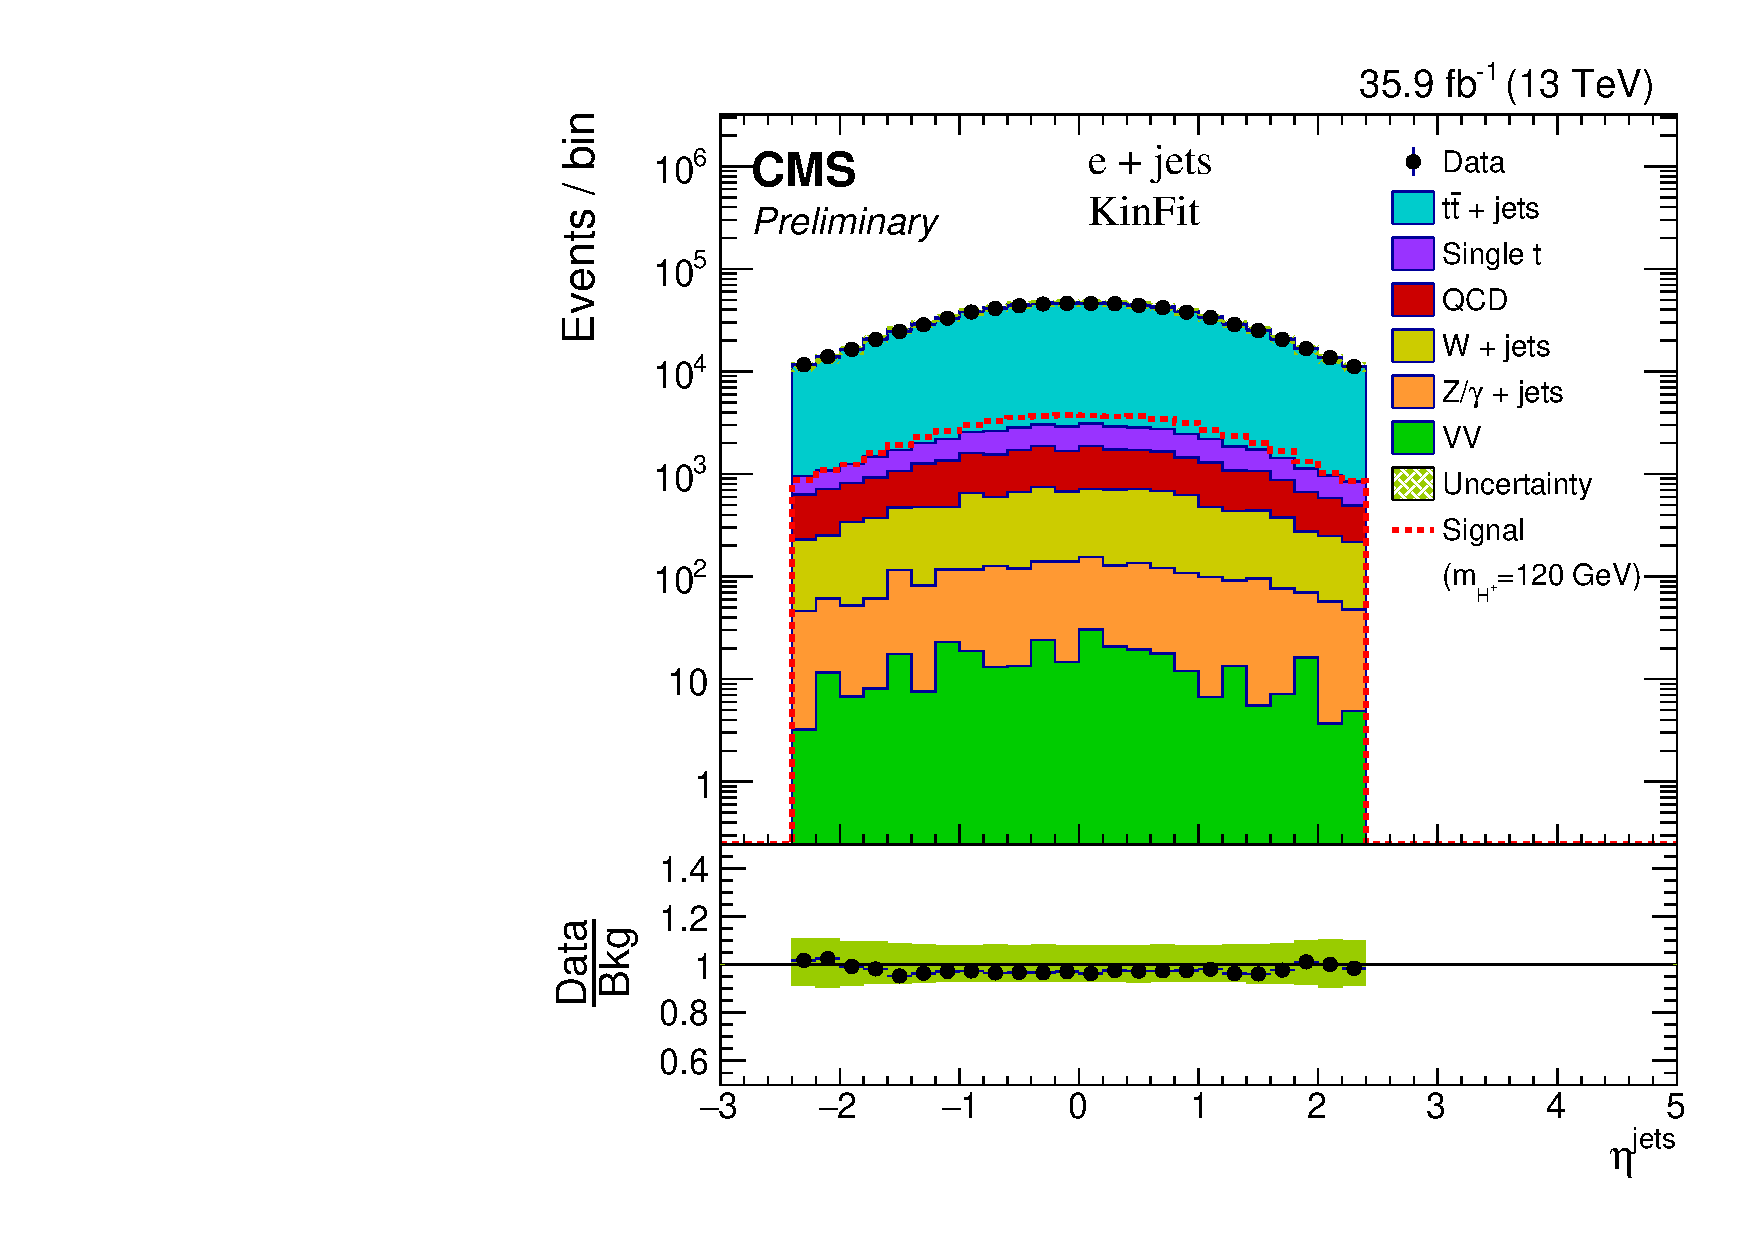
\includegraphics[width=0.40\linewidth]{Image/Electron/KinFit/eta_jet_eleKinFit.pdf}}
    \vfil
    \subfigure[jet multiplicity]{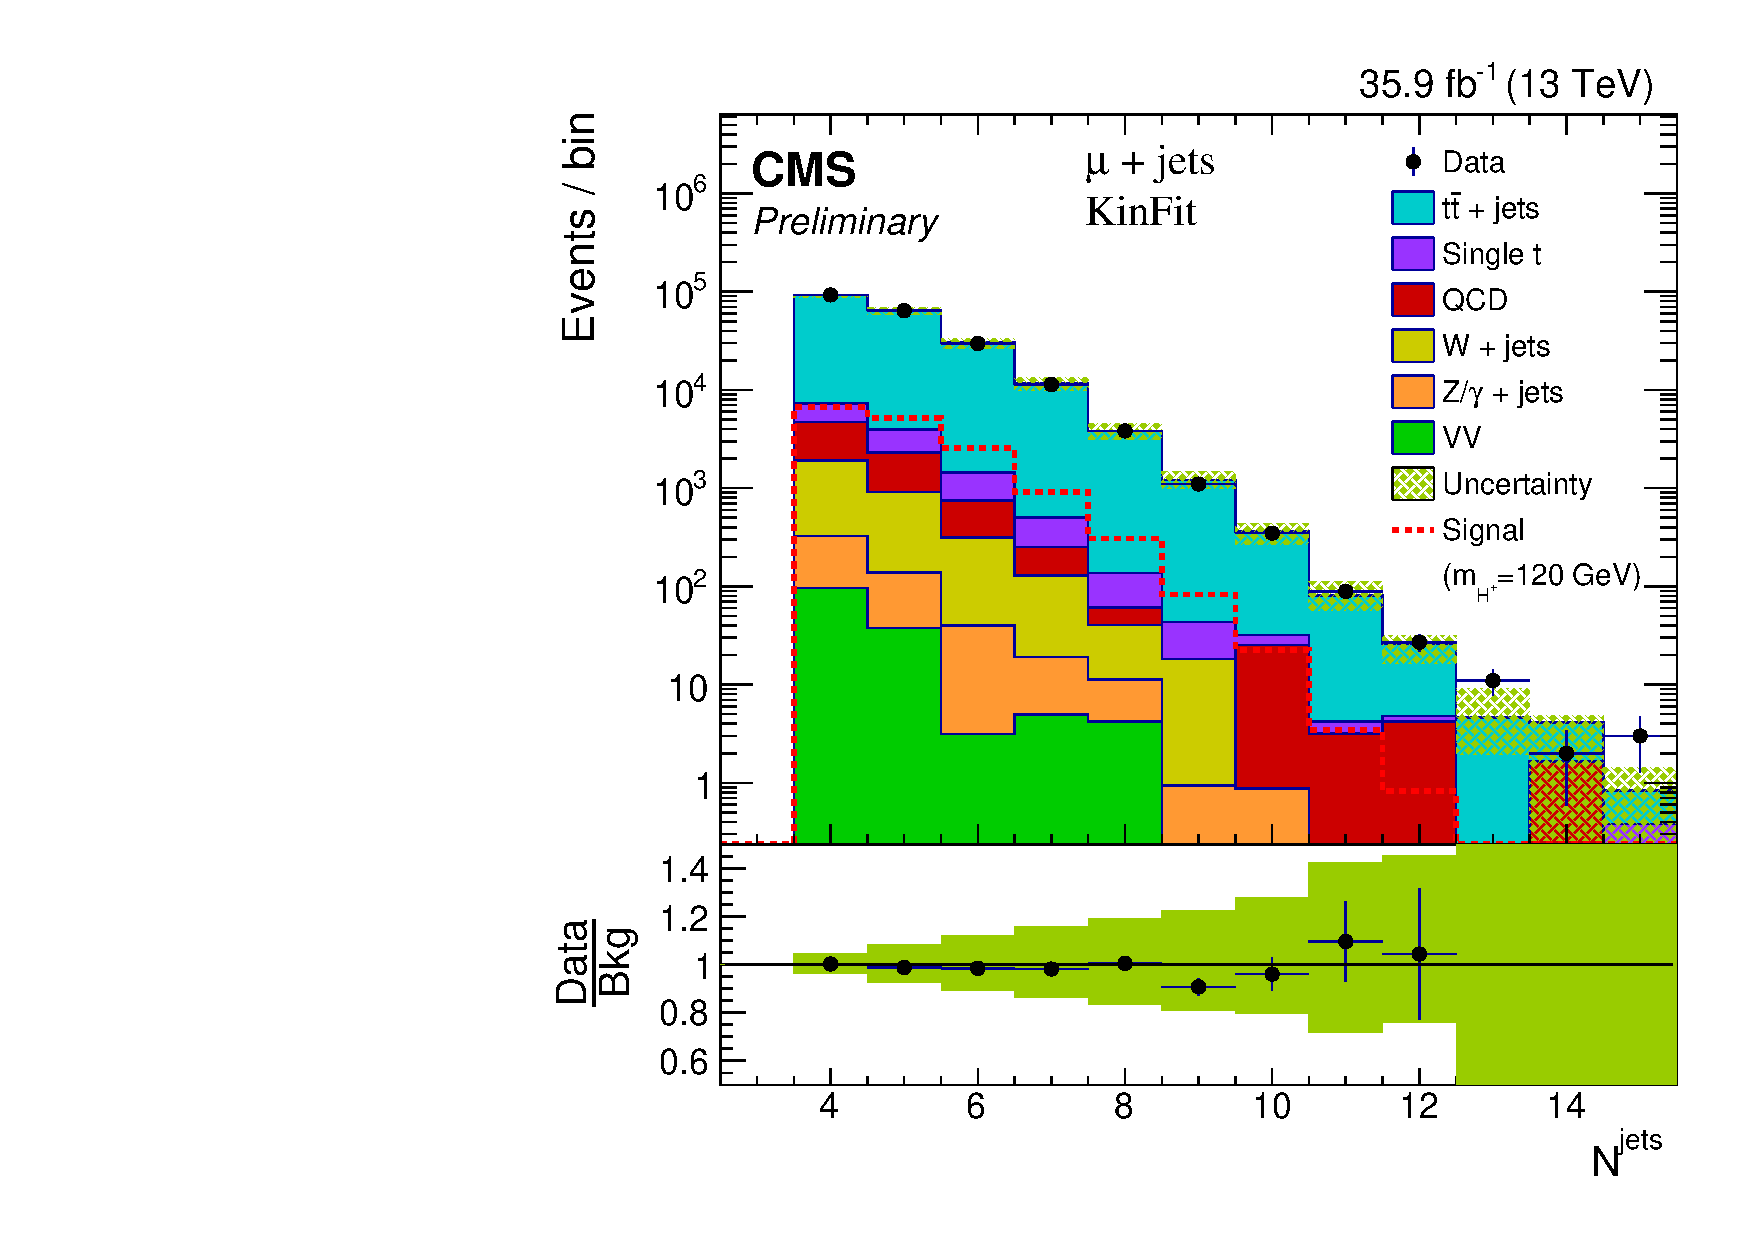
\includegraphics[width=0.40\linewidth]{Image/Muon/KinFit/final_multi_jet_muKinFit.pdf}}
    \subfigure[jet multiplicity]{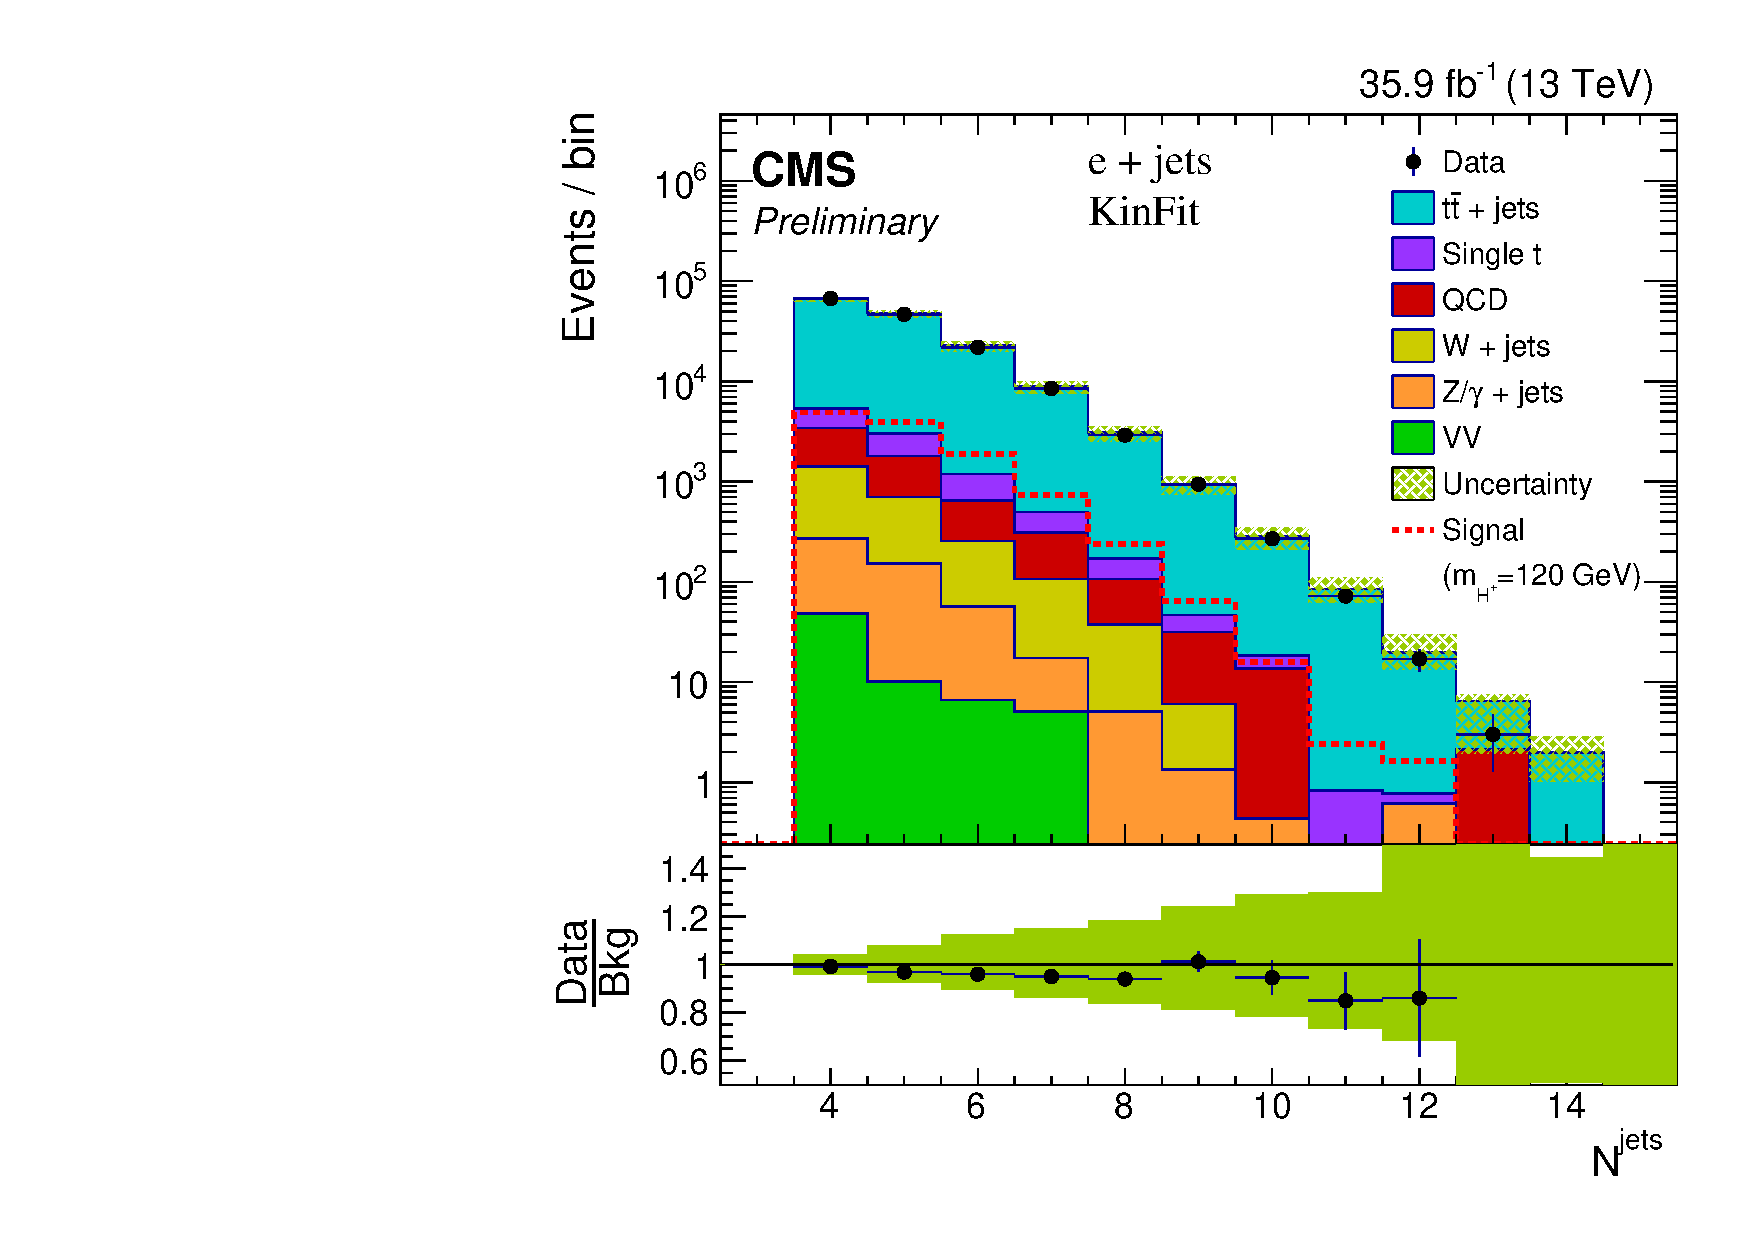
\includegraphics[width=0.40\linewidth]{Image/Electron/KinFit/final_multi_jet_eleKinFit.pdf}}
    \vfil
    \subfigure[\PQb jet multiplicity]{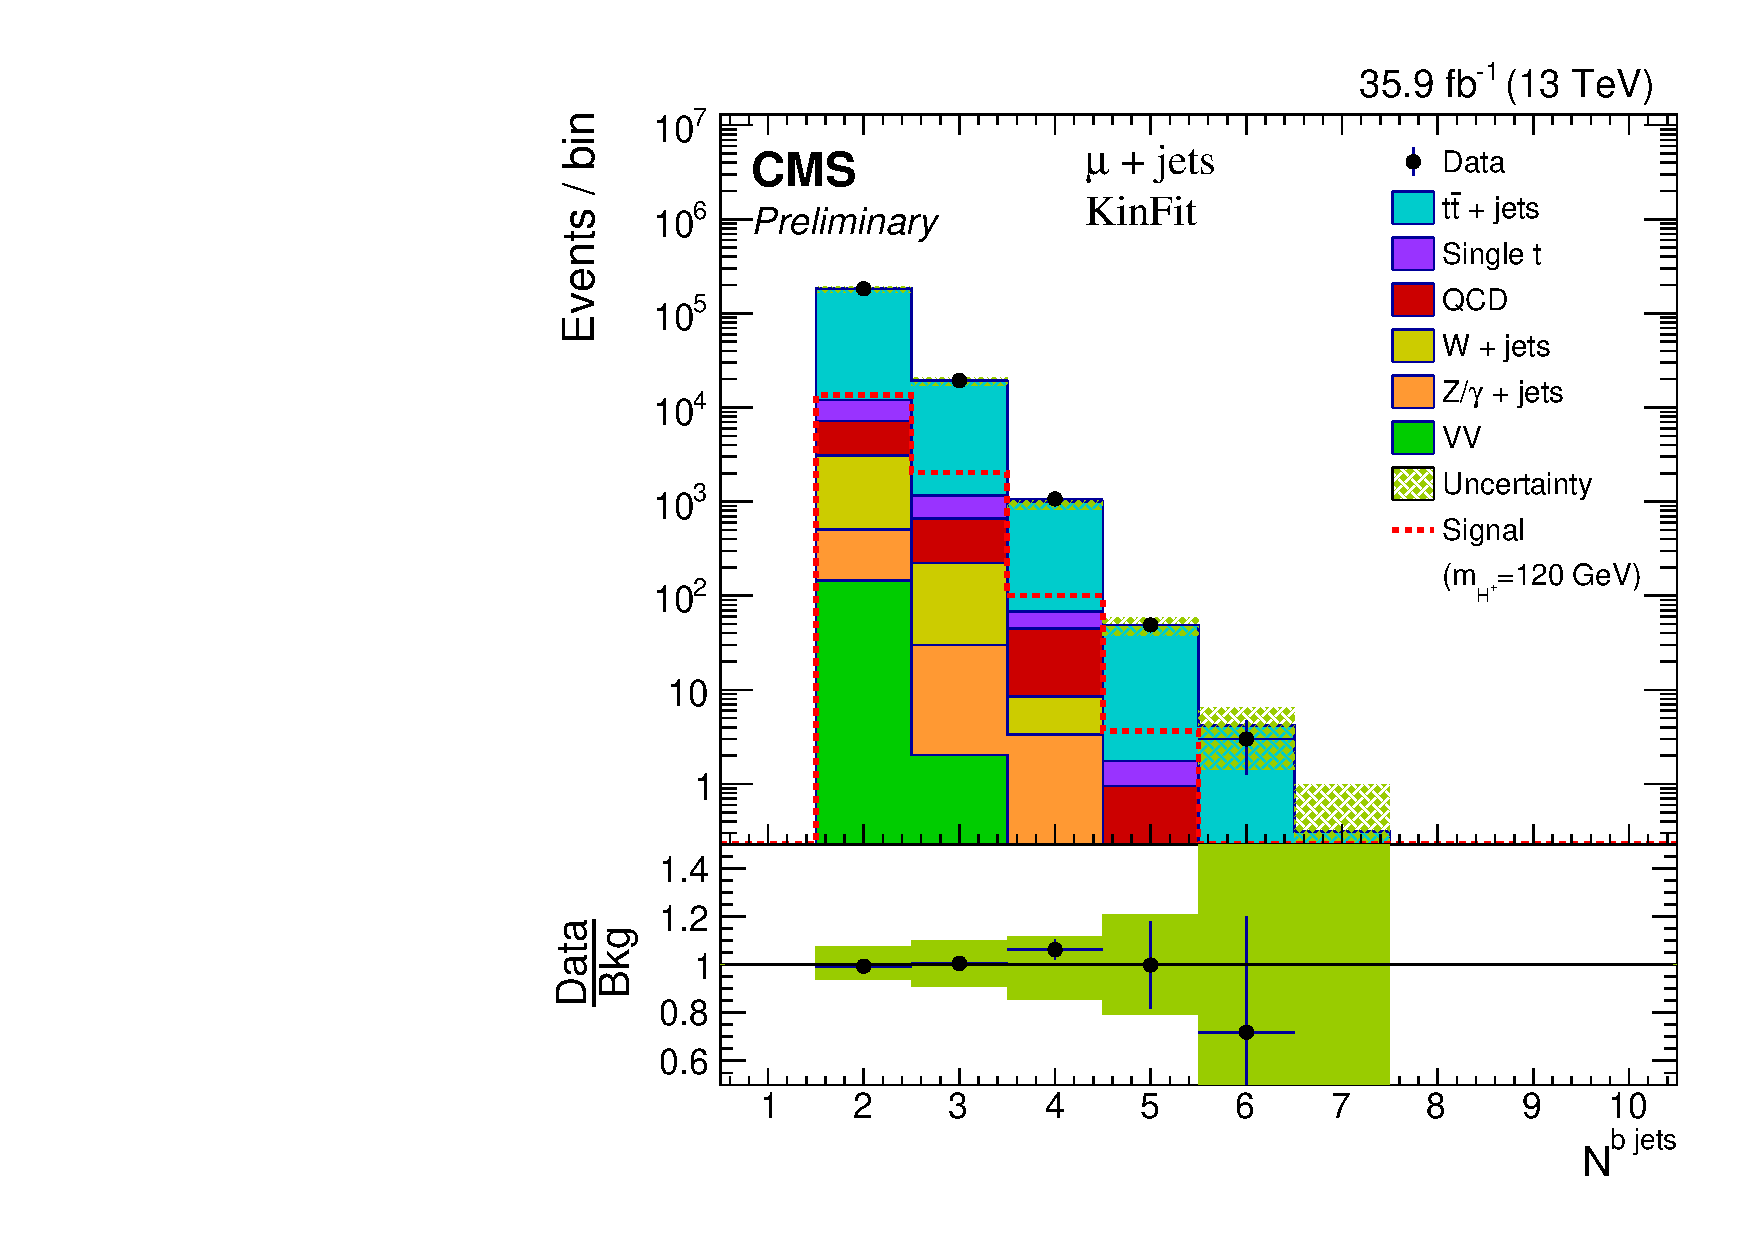
\includegraphics[width=0.40\linewidth]{Image/Muon/KinFit/CSVL_count_muKinFit.pdf}}
    \subfigure[\PQb jet multiplicity]{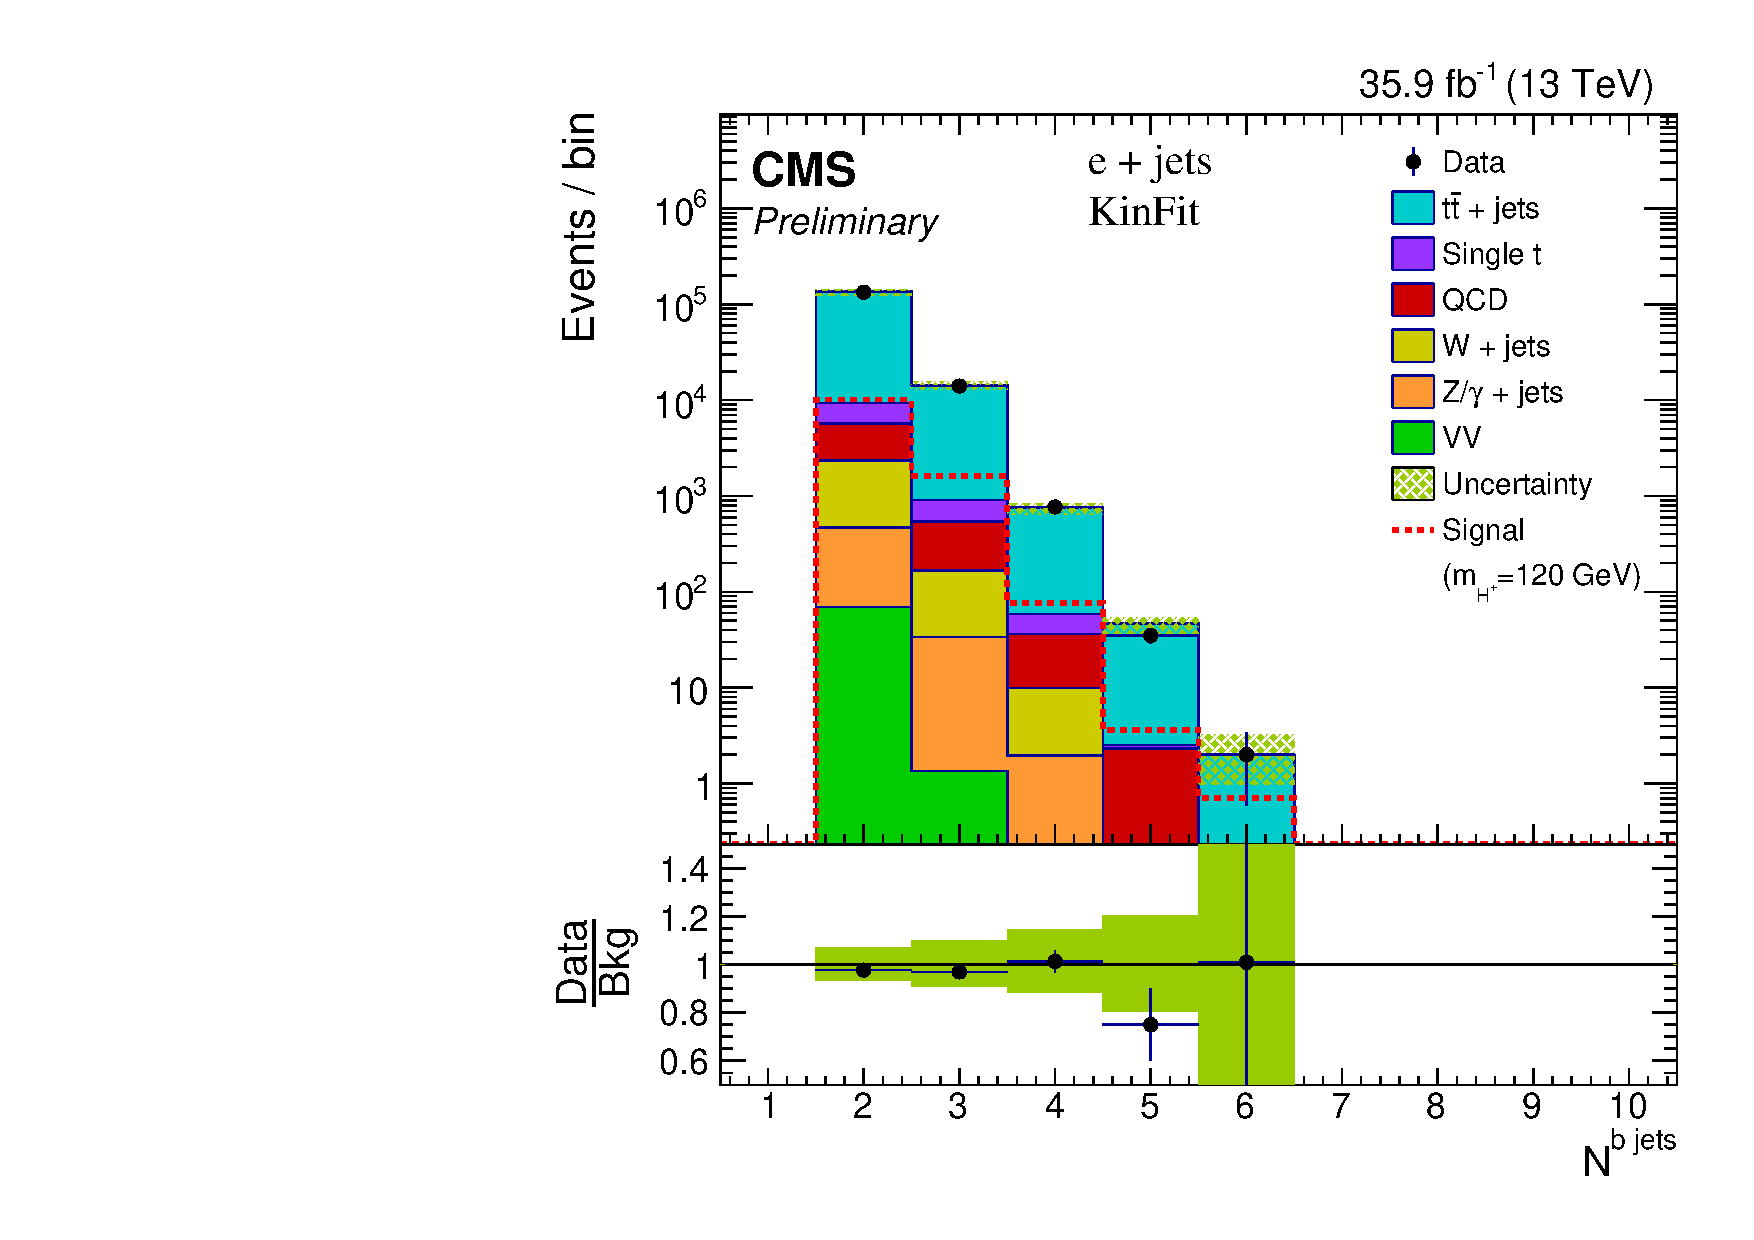
\includegraphics[width=0.40\linewidth]{Image/Electron/KinFit/CSVL_count_eleKinFit.pdf}}
    \caption{Distribution of kinematic fitted $\eta$ of jets, jet multiplicity, and \PQb jet
        multiplicity after kinematic fit selection for \mujets and \ejets channel.}
    \label{fig:kfitPlot2}
\end{figure}

\begin{figure}
    \centering  
    \subfigure[Missing transverse energy]{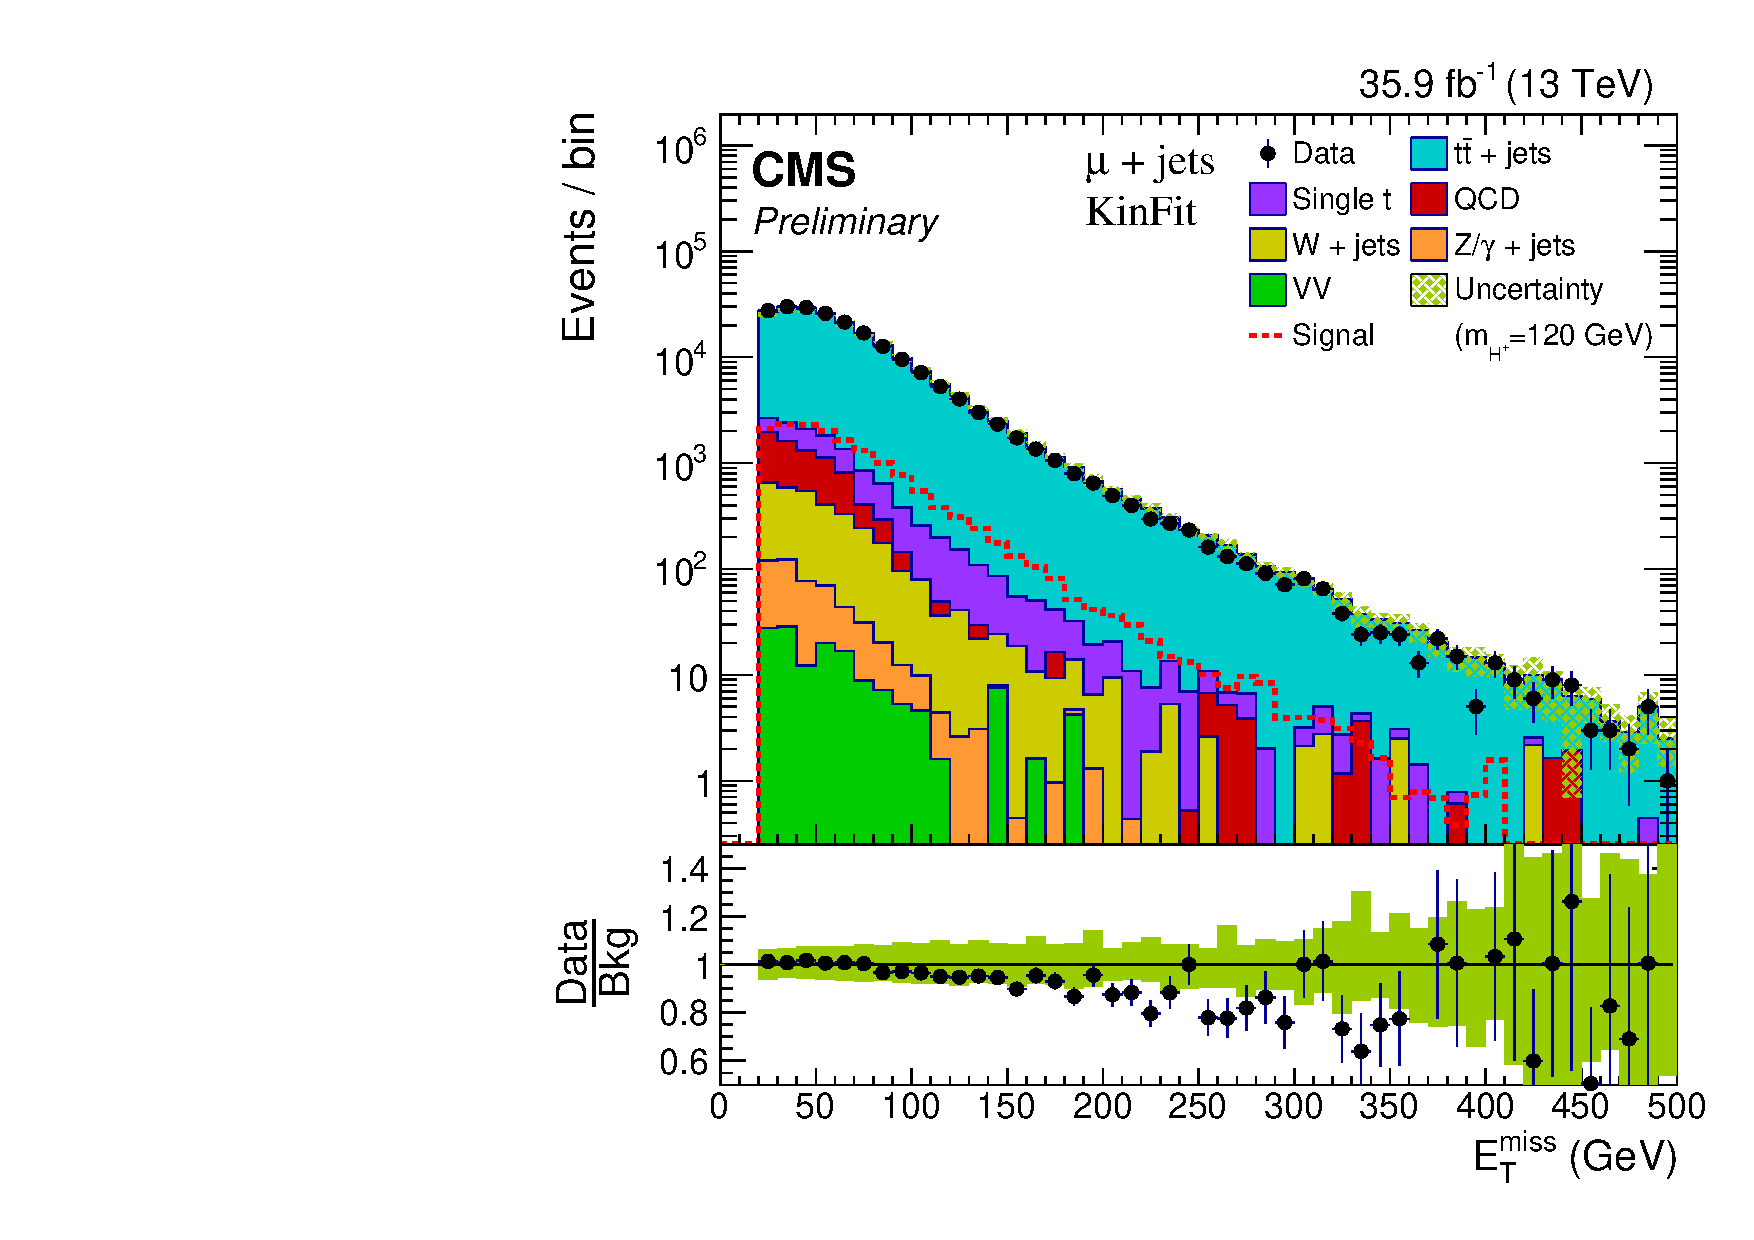
\includegraphics[width=0.45\linewidth]{Image/Muon/KinFit/final_pt_met_muKinFit.pdf}}
    \subfigure[Missing transverse energy]{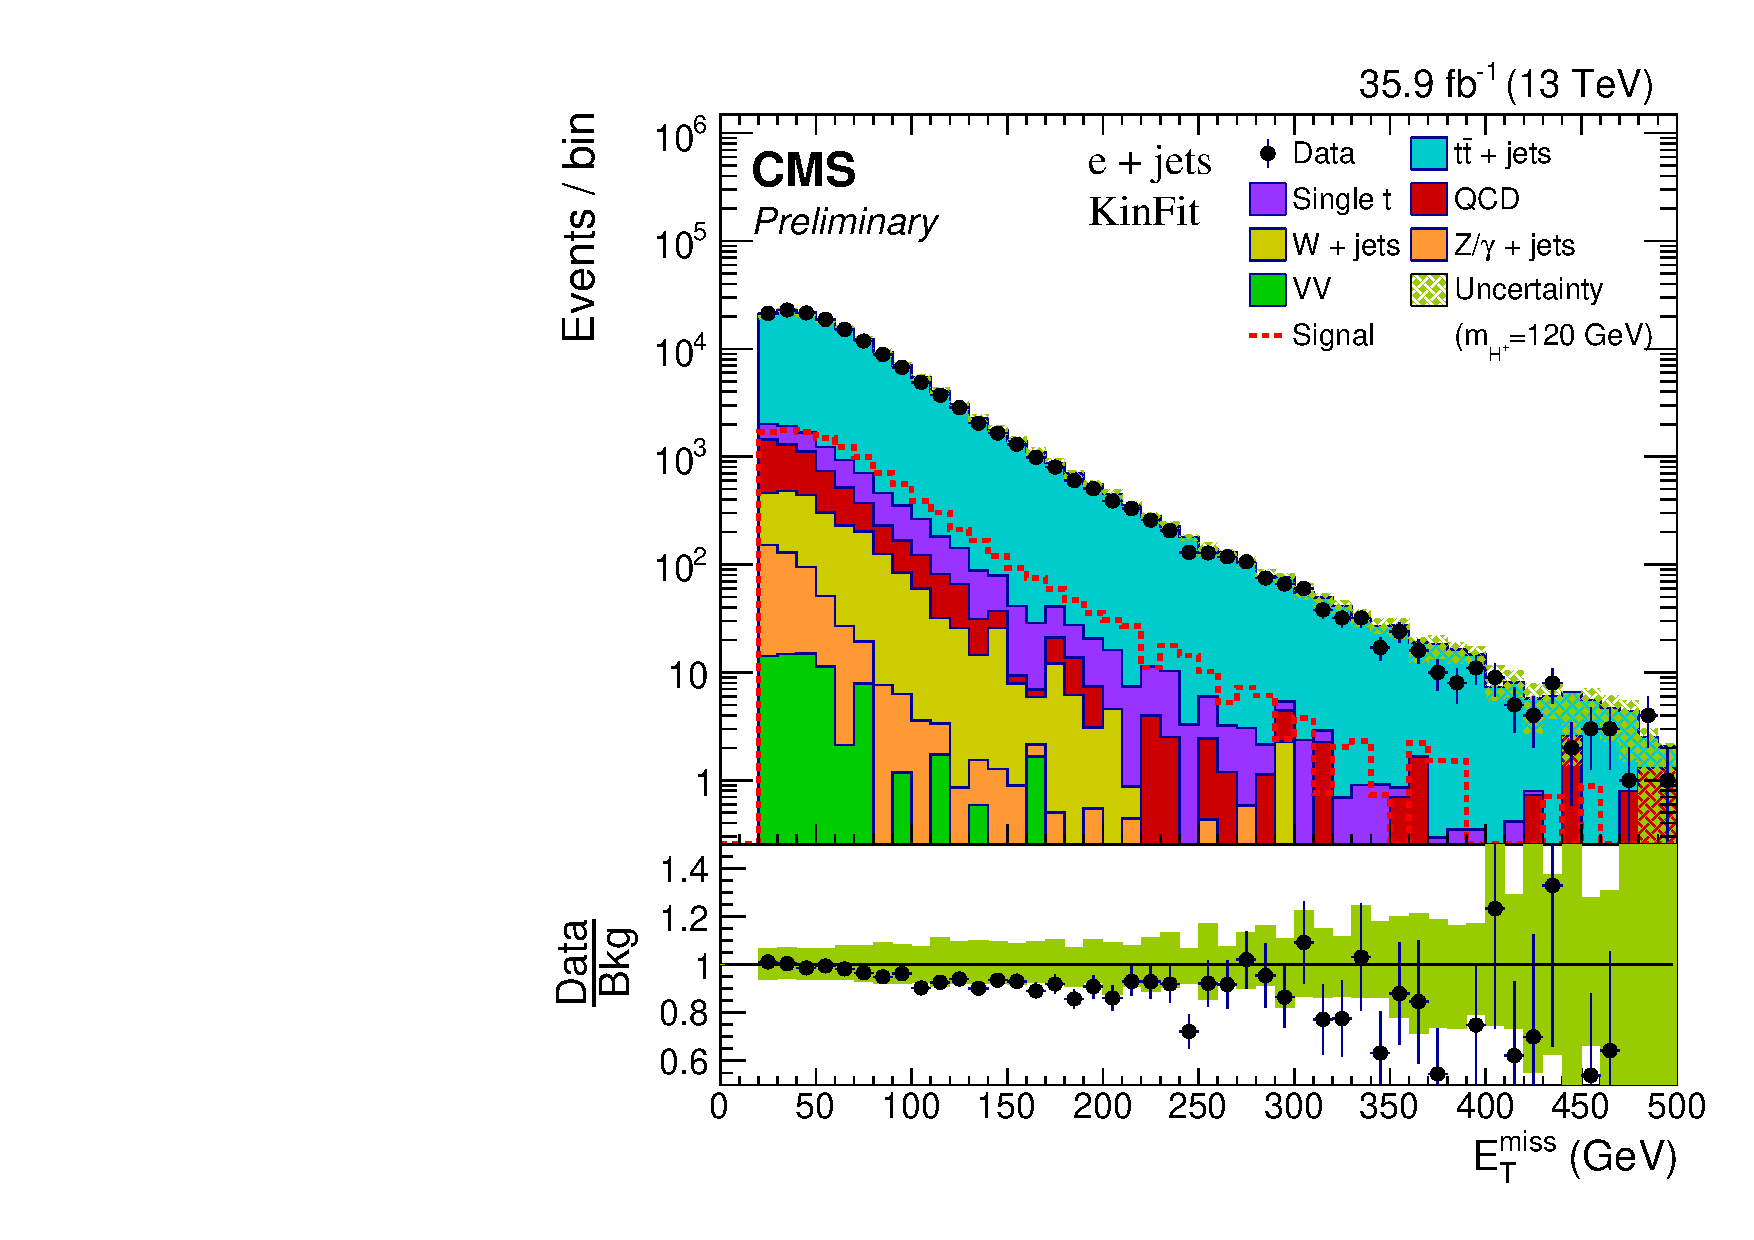
\includegraphics[width=0.45\linewidth]{Image/Electron/KinFit/final_pt_met_eleKinFit.pdf}}
    \vfil
    \subfigure[Transverse mass of \PW boson]{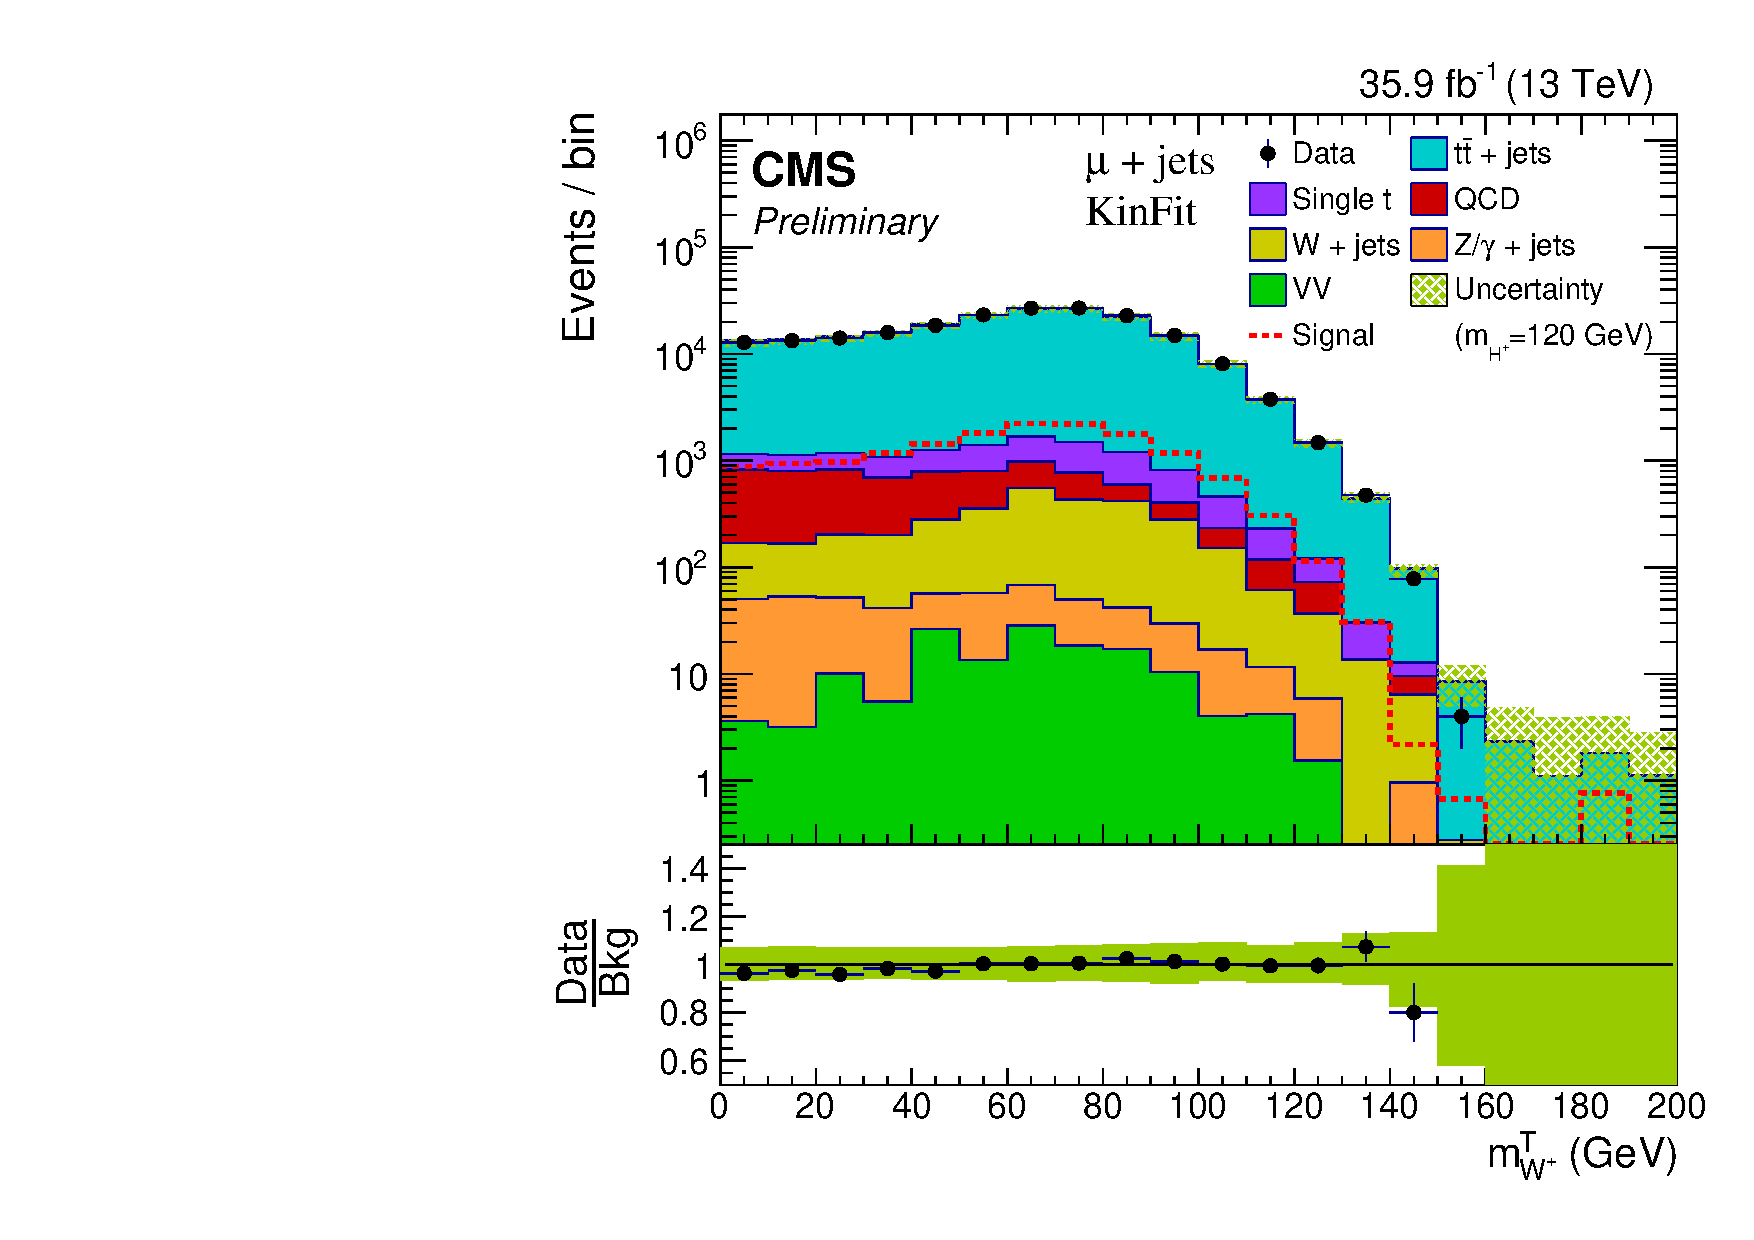
\includegraphics[width=0.45\linewidth]{Image/Muon/KinFit/wmt_muKinFit.pdf}}
    \subfigure[Transverse mass of \PW boson]{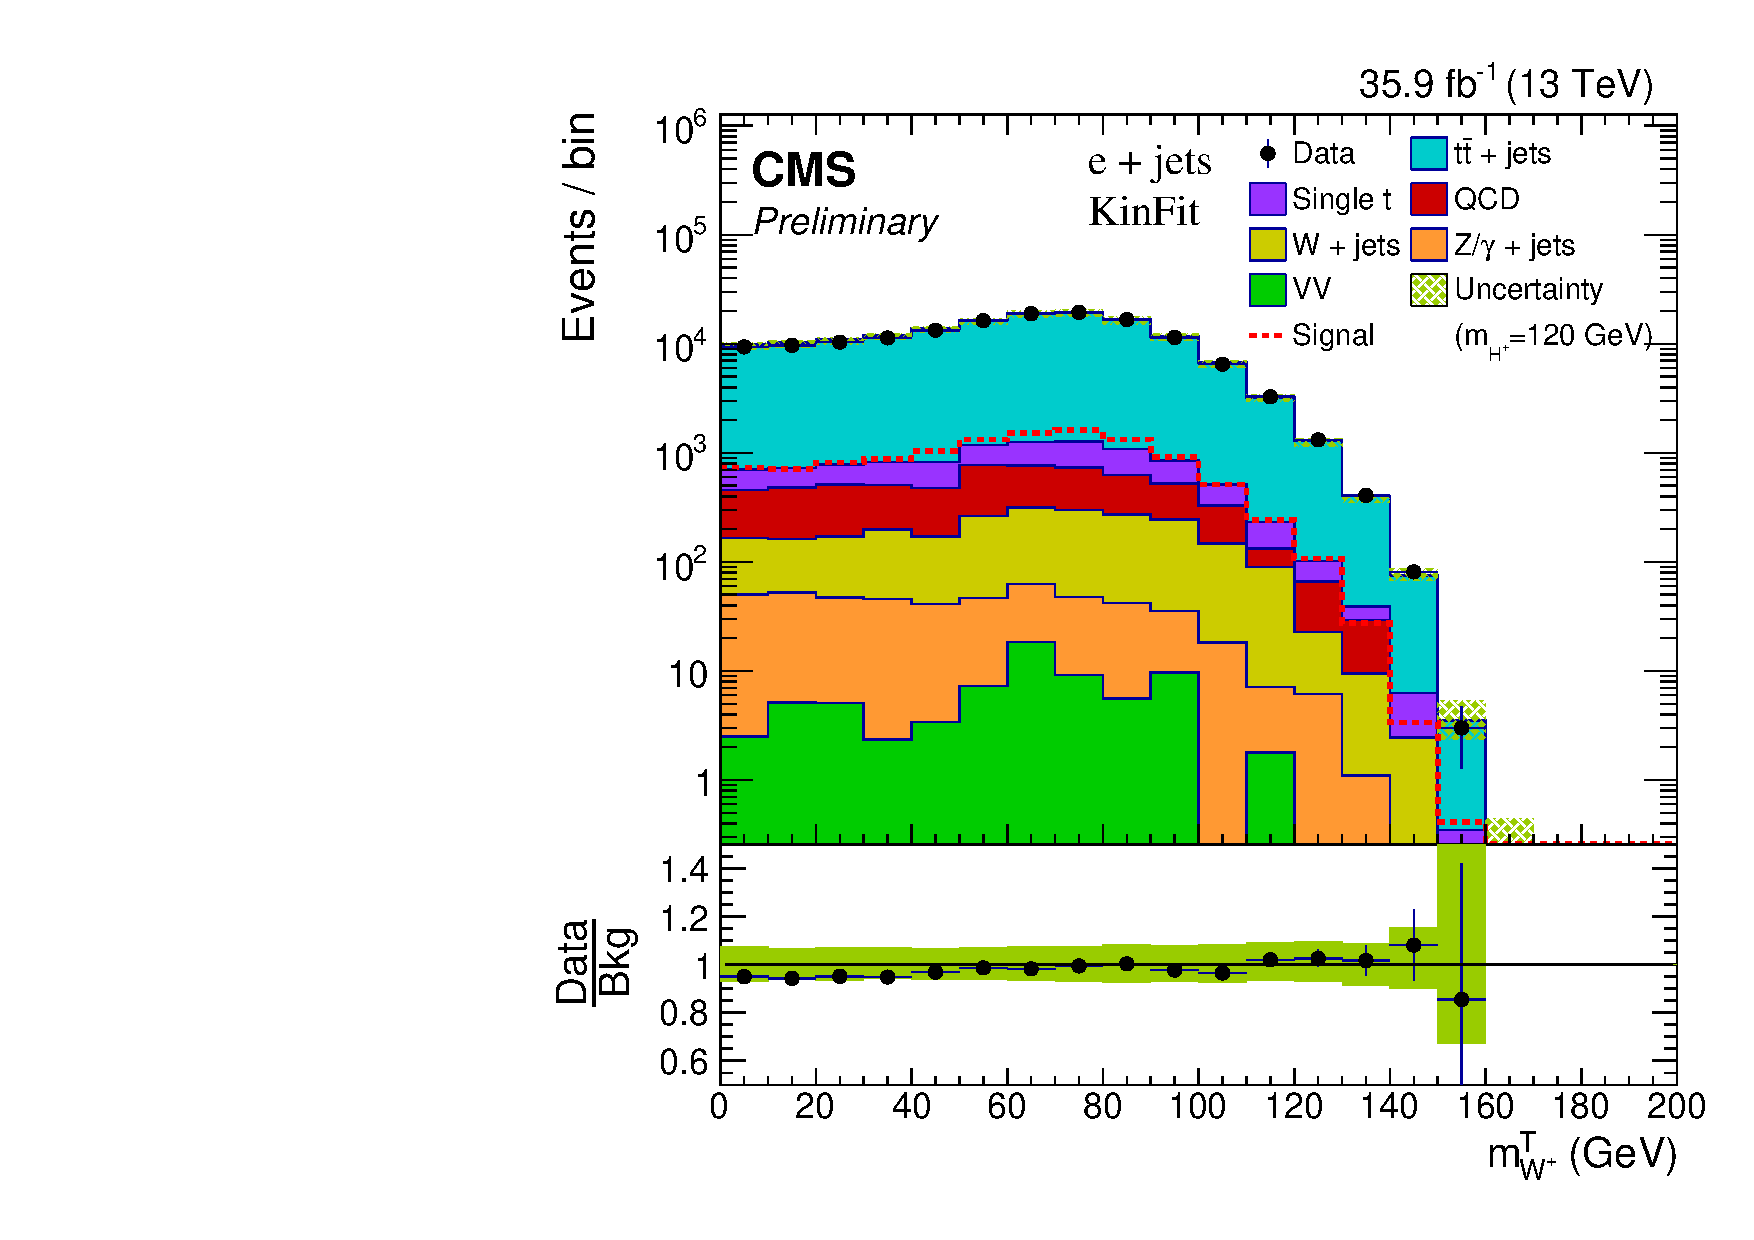
\includegraphics[width=0.45\linewidth]{Image/Electron/KinFit/wmt_eleKinFit.pdf}}
    \caption{Distribution of kinematic fitted $\MET$ and $m_{\PW^+}^{T}$ after kinematic fit selection 
	for \mujets and \ejets channel.}
    \label{fig:kfitPlot3}
\end{figure}
